\documentclass[iop,twocolappendix]{emulateapj}

\usepackage{graphicx}
\usepackage{amssymb}
\usepackage{amsmath}
\usepackage{natbib}
\usepackage{longtable}
\usepackage{footnote}
\bibliographystyle{apj}
\usepackage{helvet}
\usepackage{color}
\usepackage{afterpage}
\usepackage{float}
\usepackage{soul}
\usepackage[toc,page]{appendix}
\usepackage{chngcntr}
\usepackage[breaklinks,colorlinks,citecolor=blue,backref=section]{hyperref}

\slugcomment{Draft version \today}

\begin{document}

% names
\newcommand{\IRAS}{IRAS 16293-2422}
\newcommand{\ALMA}{Atacama Large Millimeter/submillimeter Array}
% molecules
\newcommand{\A}{CH$_3$CHO}
\newcommand{\M}{CH$_3$OH}
\newcommand{\MF}{CH$_3$OCHO}
% moments
\newcommand{\momzero}{$\mu_0$}
\newcommand{\momone}{$\mu_1$}
\newcommand{\momtwo}{$\mu_2$}
% parameters, symbols
\newcommand{\vLSR}{$v_{\mathrm{LSR}}$}
\newcommand{\dispersion}{${\sigma}_v$}
\newcommand{\restfreq}{${\nu}_0$}
\newcommand{\nuLSR}{${\nu}_\mathrm{LSR}$}
\newcommand{\Msun}{M$_{\odot}$}
\newcommand{\Mstar}{$M_{\ast}$}
\newcommand{\Menv}{$M_\mathrm{env}$}
\newcommand{\Td}{$T_d$}
\newcommand{\Flux}{F$_{\nu}$}
\def\plus{\texttt{+}}
\newcommand{\redchisq}{$\bar{{\chi}}^2$}
\newcommand{\Aul}{$A_{ul}$}
\newcommand{\Eul}{$E_{ul}$}
\newcommand{\Nthin}{$N_{ul}^\mathrm{thin}$}
\newcommand{\Ntot}{$N_\mathrm{tot}$}
\newcommand{\Trot}{$T_\mathrm{rot}$}
% units
\newcommand{\kms}{$\mathrm{km\,s^{-1}}$}
\newcommand{\Jybeamkms}{Jy\,beam$^{-1}$\,km\,s$^{-1}$}
\newcommand{\Jybeam}{Jy\,beam$^{-1}$}
% comments
\def\jessica#1{\noindent{\bf \textcolor{magenta}{[#1]}}}

% NO SPACE AT TOP OF FIGURES
\makeatletter
\setlength{\@fptop}{0pt}
\makeatother

% ADD WHITESPACE TO TABLES
\newcommand\T{\rule{0pt}{2.6ex}} % Top strut
\newcommand\B{\rule[-1.2ex]{0pt}{0pt}} % Bottom strut

%%% TITLE %%%
\title{Constructing a Python Pipeline for Analyzing Spatially Resolved ALMA Observations of IRAS 16293-2422}

%%% AUTHORS %%%
\author{J. L. Campbell\altaffilmark{1,2}}
\email{jessicalynn.campbell@mail.utoronto.ca}
\author{Magnus Persson\altaffilmark{3}}
\author{Mihkel Kama\altaffilmark{3}}

\altaffiltext{1}{Department of Astronomy \& Astrophysics, University of Toronto, Canada.}
\altaffiltext{2}{Leiden/ESA Astrophysics Program for summer Students (LEAPS), Leiden Sterrewacht (Observatory), Leiden University, The Netherlands.}
\altaffiltext{3}{Leiden Sterrewacht (Observatory), Leiden University, The Netherlands.}

%%% ABSTRACT %%%
\begin{abstract}

We discuss the results of a Python pipeline written to analyse high quality ALMA data of the deeply-embedded low-mass protostar {\IRAS}. The emission is spatially resolved, providing a unique insight into the morphology of the complex organic molecules abundant in hot corino objects. We investigate detections of 97 pure rotational transitions of {\A} (acetaldehyde), 18 transitions of {\M} (methanol), and 50 transitions of {\MF} (methyl formate) above a 5\,$\sigma$ level. Using an LTE model, acetaldehyde and methanol are found at local standard-of-rest velocities of {\vLSR} = 2.7 \kms, while methyl formate is found at {\vLSR} = 4.7 \kms. The tasks performed by the Python pipeline to analyse the data includes creating noise maps as well as integrated line intensity, velocity, and velocity dispersion maps of all detected rotational transitions. We find no trend with {\Eul} and {\vLSR} nor {\Eul} and {\dispersion}. We do however find a correlation between {\dispersion} and {\vLSR} for $v > v_\mathrm{LSR}$, and an anti-correlation for $v < v_\mathrm{LSR}$, likely the result of line-blending.  Column density maps of each detected transition (\Nthin) are also created for regions excluding absorption with the assumption that the emission is optically thin. Using the population diagram technique, which consists of plotting {\Nthin} per statistical weight as a function of the upper-level energy, total column density (\Ntot) and rotational (excitation) temperature (\Trot) maps are created for the three molecules. Restricting these maps to 5\,$\sigma$ measurements using the fit uncertainties still result in regions of non-physical (i.e., negative) temperatures and unusually high column densities, so they are confined to regions satisfying $0\,\mathrm{K} < T_\mathrm{rot} < 2500\,\mathrm{K}$. Further investigation is required to determine whether this is the result of the gas being in non-LTE, in which case the population diagram technique would be an inadequate approximation. Analysing the spatial distribution of the emission in the {\Ntot} and {\Trot} maps indicates that, while acetaldehyde and methyl formate have somewhat extended emission, methanol is found to be particularly compact. This may however be due to the lower detection rate of methanol. The combination of line blending and ALMA's small beam size cannot explain the extent to which observed {\Ntot} are higher than previously found, thus further investigation is required. The median {\Trot} found for acetaldehyde is 254\,K, and is consistent with previous studies. Median {\Trot} values for methanol and methyl formate are 1,189\,K and 307\,K, respectively.

\end{abstract}

\maketitle

%%% INTRODUCTION %%%
\section{Introduction}
\label{sec:introduction}

Low-mass stars are believed to form through the gravitational collapse of over-densities in the interstellar medium (ISM) located in the coldest and densest regions of molecular clouds \citep[e.g.,][]{Myers1985}. The details of the subsequent evolution of these so-called dense cores from starless to their protostellar counterparts remains one of the largest controversies in star formation research, establishing the need for both observational and theoretical studies of young stellar objects (YSOs). Understanding the chemical enrichment that occurs as dense cores evolve is an active area of research as its role in the star formation process is poorly understood. Chemically-rich environments around some YSOs called ``hot corinos'' are the low-mass counterpart to high-mass ``hot cores'' that are characterized by warm temperatures ($T\,{\geq}\,100$~K), high densities ($n\,{\geq}\,10^{6}$\,cm$^{-3}$) \citep{Cazaux2003}, and a rich inventory of molecular species not abundant in dark molecular clouds \citep{Walmsley1992}. Continuum studies of chemically-rich protostellar envelopes have indicated a spatial offset in the emission of complex organic molecules from the peak of the dust continuum emission in some YSOs \citep[e.g.,][]{Chandler2005}, suggesting the need for an alternative explanation to the hot corino hypothesis to explain the origin of complex organics in YSO environments. Additionally, the question of whether observed complex organics are first generation molecules that are created in icy dust-grain mantles and are subsequently sublimated into the gas phase, or second generation molecules that are the result of grain-mantle evaporation followed by rapid gas phase reactions, remains an open debate today for many molecular species \citep{Bisschop2008}. 

%%% Summary of Observations Table %%%
\begin{deluxetable*}{lccccc}
\tablecolumns{6}
\tablecaption{Summary of ALMA Observations}
\tablehead{
\colhead{spw} & \colhead{$\nu$} & \colhead{{\restfreq}} & \colhead{${\Delta}v$} & \colhead{$\Omega$} &  \colhead{Sensitivity} \\
\colhead{Sidebands} & \colhead{(GHz)} & \colhead{(GHz)} & \colhead{(\kms)} & \colhead{(arcsec$^2$)} &  \colhead{(Jy\,beam$^{-1}$\,channel$^{-1}$)} \\
\colhead{(1)} & \colhead{(2)} & \colhead{(3)} & \colhead{(4)} & \colhead{(5)} &  \colhead{(6)} 
}
\startdata
0a & 703.25 -- 704.18 & 703.3125 & 0.416 & 0.053 & 0.017 \\
0b & 704.18 -- 705.10 & 703.3125 & 0.419 & 0.054 & 0.121 \\
1a & 692.16 -- 691.12 & 692.2375 & 0.423 & 0.057 & 0.093 \\
1b & 691.23 -- 690.30 & 692.2375 & 0.424 & 0.057 & 0.095 \\
2a & 690.36 -- 689.43 & 690.4375 & 0.424 & 0.057 & 0.092 \\
2b & 689.43 -- 688.50 & 690.4375 & 0.425 & 0.058 & 0.091 \\
3a & 688.36 -- 687.43 & 688.4375 & 0.426 & 0.059 & 0.094 \\
3b & 687.43 -- 686.50 & 688.4375 & 0.426 & 0.059 & 0.091
\enddata
\label{table:observations}
\end{deluxetable*}

%%% Summary of Detected Transitions Table %%%
\begin{deluxetable*}{lcccc}
\tablecolumns{5}
\tablecaption{Summary of Detected Transitions}
\tablehead{
\colhead{Molecular} & \colhead{$n_\mathrm{lines}$} & \colhead{$E_{ul}$} & \colhead{$A_{ul}$} & \colhead{$g_{ul}$} \\
\colhead{Species} & \colhead{} & \colhead{(K)} & \colhead{(s$^{-1}$)} & \colhead{} \\
\colhead{(1)} & \colhead{(2)} & \colhead{(3)} & \colhead{(4)} & \colhead{(5)}
} 
\startdata
\A & 97 & 69.48 -- 998.81 & 4.25${\times}10^{-8}$ -- 1.13${\times}10^{-2}$ & 30--170 \\
\M & 18 & 154.25 -- 990.87 & 2.71${\times}10^{-9}$ -- 1.88${\times}10^{-3}$ & 17--62 \\
\MF & 50 & 257.75 -- 998.82 & 5.50${\times}10^{-6}$ -- 4.86${\times}10^{-3}$ & 74--218 
\enddata
\label{table:detections}
\end{deluxetable*}

The connection between various molecular species has previously been studied by comparing molecular abundances in a large number of sources using single-dish radio telescopes \citep[e.g.,][]{vanderTak2000}. More recently, the high spatial resolution provided by radio interferometry has made studying the spatial distribution of molecular species possible, which allows for a better identification of where the emission is coming from \citep[e.g.,][]{Bisschop2008}. Spatially resolved molecular emission could not only assist in elucidating the origin of the chemical enrichment of the gas phase (i.e., whether complex molecules are first- or second-generation species), but also in allowing for a test of the hot corino hypothesis by searching for spatial correlations with continuum emission, protoplanetary disks, outflows, or other energy sources which could be (shock-) heating the gas. Studies of complex organics in star forming regions also serves as useful tracers for the physical conditions of star forming environments, such as their temperature, density, and velocity profiles, as well as indicators of their lifetime, evolutionary phase, and chemical complexity \citep{Herbst2009}.

In this paper, we discuss a Python pipeline that was constructed to analyze high quality radio data of chemically-rich sources with spatially-resolved emission and an abundance of molecular lines. We review the results of {\IRAS} using publicly available {\ALMA} (ALMA) data, while focusing on a small subset of the molecular species present: acetaldehyde (\A), methanol (\M), and methyl formate (\MF). Details on the {\IRAS} source are discussed in Section \ref{sec:IRAS}, while ALMA observations are outlined in Section \ref{sec:observations}. The details of the Python pipeline are presented in Section \ref{sec:pipeline}. We discuss the results in Section \ref{sec:discussion}, which includes some future work discussion on features that will be implemented into the Python pipeline. A summary is presented in Section \ref{sec:summary}, which includes a list of the tasks that the Python pipeline completes to analyse the high quality ALMA data.

\begin{figure*}[t]
\begin{center}
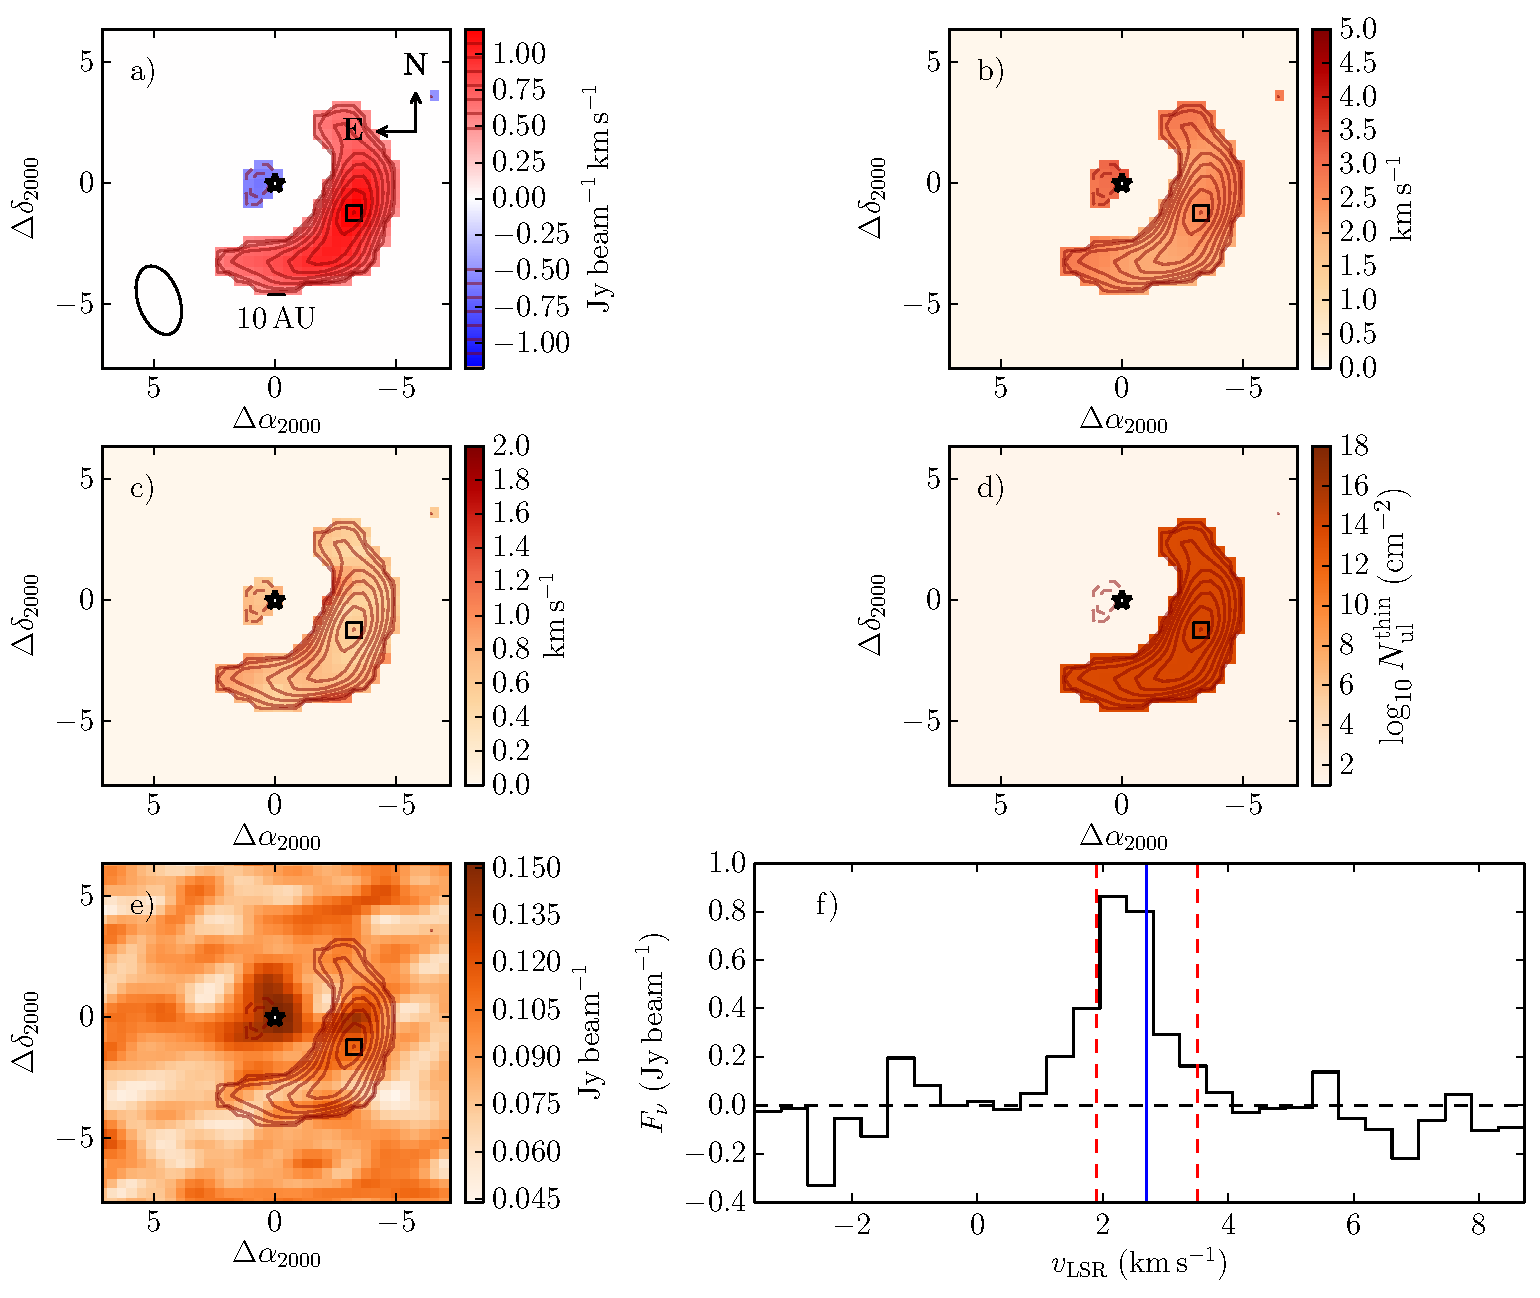
\includegraphics[width=15cm]{Acetaldehyde_(14-510-1).pdf}
\caption{Emission of a rotational transition of Acetaldehyde in IRAS B with Quantum Numbers (21 318 2), an upper-level energy {\Eul}=235.36 K, and an Einstein A coefficient {\Aul} = 3.49${\times}10^{-4}$\,s$^{-1}$. The (black) star symbol indicates the pointing position of the IRAS B protostar, and the (black) square indicates the region with the strongest emission, corresponding to the spectrum shown in (f). Contours are those of the moment 0 map. (a) Moment 0 (\momzero) map, displaying the integrated line intensity. The beam size is shown in the bottom left corner, and 10 AU is shown to scale. (b) Moment 1 (\momone) map, displaying the average velocity of the emission. (c) Moment 2 (\momtwo) map, displaying the velocity dispersion of the emission. (d) Column density (\Nthin) of the transition. Note that {\Nthin} was determined for regions excluding absorption corresponding to the blue spatial region in (a). (e) Noise (rms) map of the spectral window. (e) Emission spectrum of the brightest spatial pixel, indicated by the (black) square. The (blue) solid vertical line is the {\vLSR} of the molecule, and the (red) dashed vertical lines are the ${\pm}\,1.5\,\sigma$ velocity range that was used to calculate the maps in (a) -- (d).}
\label{fig:exmaps}
\end{center}
\end{figure*}

%%% IRAS16293-2422 %%%
\section{IRAS16293-2422}
\label{sec:IRAS}

{\IRAS}, hereafter IRAS 1624, is a solar-type protostar in its early stage of formation located in the $\rho$ Ophiuchi molecular cloud complex in the Ophiuchus molecular cloud. This exemplary candidate for astrochemical studies has a rich inventory of molecular species \citep[e.g.,][]{Walker1986, Bisschop2008} and is a deeply-embedded Class 0 protostar, which are protostars defined to be in their earliest stage of formation such that {\Mstar} $<<$~{\Menv} and {\Td} $\lesssim$~20 K \citep{Andre1993}. This source was one of the first protostellar systems identified as a binary candidate using dust continuum maps \citep{Mundy1986}, indicating a Southeastern ``A'' source and a Northwestern ``B'' source, hereafter IRAS A and IRAS B, respectively. The two components of IRAS A have a source separation of 0$\farcs$3, with IRAS B having a separation from IRAS A of 5\,$\arcsec$ \citep{Mundy1986, Wootten1989}. At a distance of 160 parsecs, these angular separations correspond to physical distances of 48 AU and 800 AU, respectively. IRAS B is located at a right ascension of 16$^\mathrm{h}$32$^\mathrm{m}$22$^\mathrm{s}$.61597 and a declination of $-$24$\degr$28$\arcmin$32$\farcs$496462.

Both of the IRAS A and B components have been found to contain a wealth of molecules in their circumstellar envelopes \citep[e.g.,][]{Bisschop2008}. However there remain important differences between the two sources. Spectral observations by \citet{Jorgensen2011} found IRAS A and IRAS B to have average local-standard-of-rest velocities (\vLSR) of 3.2 {\kms} and 2.7 {\kms}, and average velocity dispersions (\dispersion) of 2.6 {\kms} and 1.9 {\kms}, respectively. Using a standard T test for distributions with different variances, they found the {\vLSR} and {\dispersion} distributions to be significantly different. \citeauthor{Jorgensen2011} also found many Nitrogen- and Sulfur-bearing species to be predominantly detected towards IRAS A, with Oxygen-bearing complex organics to be more strongly detected towards IRAS B. The wealth of differences between the two sources indicates strong evidence for different physical environments likely to the result of being at different stages of evolution or evolving in different environments. IRAS A is known to be driving two bipolar outflows \citep[see][]{Mundy1992, Walker1988}, while IRAS B presents clear indications of infall \citep[e.g.,][]{Pineda2012}. While IRAS A is generally agreed upon to be a protostar, the nature of IRAS B remains debated. Some authors have suspected IRAS B to be a prestellar core (i.e., a starless core expected to form a protostar) \citep{Chandler2005}, while others argue that IRAS B is a T Tauri star \citep{Stark2004}.

IRAS 1624 presents itself as a unique opportunity to study the earliest stages of the formation of (high multiplicity) protostellar systems, infalling circumstellar envelopes, molecular outflows and shocks, as well as the wealth of molecular chemistry present in these environments.

%%% OBSERVATIONS %%%
\section{ALMA Observations}
\label{sec:observations}

Spectral observations of IRAS 1624 were taken with the {\ALMA} (ALMA) on April 16, 2012. The antenna configuration used was such that 15 antennas covered 105 independent baselines ranging from 26 -- 402 m. The data was obtained in four spectral windows (spw), each one having an ``a'' and ``b'' sideband, resulting in 1900 spectral channels and a 1.86 GHz bandwidth in each spw. With a spectral resolution of ${\Delta}{\nu} = 976.46$ kHz and rest frequencies ranging from {\restfreq} = 688.4375 -- 703.3125 GHz, the corresponding velocity resolution ranged from ${\Delta}v$ = 0.416 -- 0.426 \kms. To estimate the level of noise in each spw, the baseline rms was measured in frequency ranges where no emission could be seen by eye for each independent spw. The sensitivity of the observations ranged from 0.017 -- 0.121 Jy\,beam$^{-1}$\,channel$^{-1}$. Table \ref{table:observations} summarizes the ALMA observations. 

%%% PYTHON PIPELINE %%%
\section{Constructing a Python Pipeline}
\label{sec:pipeline}

To analyze the high spectral and spatial resolution data provided by ALMA, a pipeline was written in Python to perform several tasks; this section outlines these tasks. Section \ref{subsec:queries} discusses the catalogs used to determine molecular emission lines present in the data, with the determination of detections discussed in Section \ref{subsec:detections}. The analysis of moment maps are outlined in Section \ref{subsec:maps}, with moment 0 maps discussed in Section \ref{subsubsec:mom0}, moment 1 maps in Section \ref{subsubsec:mom1}, and moment 2 maps in Section \ref{subsubsec:mom2}. The use of the population diagram technique is outlined in Section \ref{subsec:popdiagram}, which includes the total column density and the rotational temperature of each molecule. 

The current section outlines the details of the pipeline in the context of three complex organic molecules: acetaldehyde (\A), methanol (\M), and methyl formate (\MF). 

%%% JPL AND CDMS QUERIES %%%
\subsection{JPL and CDMS Queries}
\label{subsec:queries}

To determine pure rotational molecular transitions that are present in the observed frequency ranges of each spw, NASA's Jet Propulsion Laboratory (JPL) Molecular Spectroscopy database\footnote{\url{http://spec.jpl.nasa.gov/}} as well as the Cologne Database for Molecular Spectroscopy (CDMS) database\footnote{\url{https://www.astro.uni-koeln.de/cdms/catalog}} were both queried using a Python code written by Sebastien Maret and Pierre Hily-Blant, complemented with another written by Mihkel Kama. The Splatalogue database for Astronomical Spectroscopy\footnote{\url{http://www.splatalogue.net}} was not used to query the JPL and CDMS catalogs since many transitions were found to be missing, likely because the most updated databases were not available with Splatalogue at that time. Constraints on the Einstein A coefficient ({\Aul}; related to the rate of spontaneous emission) and the upper-level energy used were {\Aul} $> 10^{-5}$\,s$^{-1}$ and {\Eul} $< 1000$\,K. Energies in units of Kelvin were converted into units of cm$^{-2}$ using the relationship $E(\mathrm{K}) = 10^{-2} (k/hc) E(\mathrm{cm^{-2}})$. A total of 220 acetaldehyde, 32 methanol, and 116 methyl formate rotational transitions were found in the frequency ranges covered by the observations.

%%% SOURCE DETECTIONS %%%
\subsection{Detections}
\label{subsec:detections}

A Local Thermodynamic Equilibrium (LTE) model was used on a few averaged spectra to estimate the {\vLSR} of each molecule. While acetaldehyde and methanol were found to have local standard-of-rest velocities of {\vLSR} = 2.7 {\kms} that agree with \citet{Jorgensen2011}, methyl formate was found at {\vLSR} = 4.7 \kms. Using these source velocities, the rest frequency of each molecular transition (\restfreq) was converted to a local standard-of-rest frequency (\nuLSR) following the radio definition,

\begin{align} \label{eq:radio}
{\nu}_\mathrm{LSR} = \left( 1 - \frac{v_\mathrm{LSR}}{c} \right) {\nu}_0\,,
\end{align}

{\noindent}which was then used to search for the location of the emission lines in the data. Assuming a FWHM of 1.9 {\kms} \citep{Jorgensen2011} for IRAS B, the line identification and analysis was made over a velocity interval of $\pm$\,1.5\,$\sigma$ about the measured systemic velocity of each emission line, which corresponds to a velocity range of $\pm$ 2.42 \kms. Converting the dispersion in velocity to frequency via

\begin{align}
{\sigma}_{\nu} = \left( \frac{{\sigma}_v}{c} \right) {\nu}_\mathrm{LSR}\,,
\end{align}

{\noindent}the frequency range within which the molecular transition is located was determined. Once the location and frequency range of each emission line was determined, the data was converted into a local standard-of-rest velocity using Equation \ref{eq:radio}. 

Possible line blending of crowded molecular emission lines was an important obstacle in determining the frequency/velocity range defined to encompass each emission line. While we assume a constant velocity dispersion across the entire source, performing more rigorous LTE modeling in various regions of the source would help to determine the linewidth of each line while adjusting for possible spatial variations and may help to correct for possible line blending. \citet{Jorgensen2011} find average FWHM values to vary from $\sim$ 0.5 {\kms} to $\sim$ 5.5 {\kms} for IRAS B, indicating a clear spatial variation in linewidth. 

We set a signal-to-noise ratio (SNR) $> 5$ in integrated line intensity ($W$) for a source detection (see Equation \ref{eq:W}). We detect 97/220 (44\%) acetaldehyde transitions, 18/32 (56\%) methanol transitions, and 50/116 (43\%) methyl formate transitions above the 5\,$\sigma$ level. The transitions of acetaldehyde cover excitation energies from 69\,K to 999\,K, with methanol covering 154\,K to 991\,K and methyl formate from 258\,K to 999\,K. The median excitation energy of acetaldehyde detected was 586\,K, with that of methanol being 742\,K and 483\,K for methyl formate. Table \ref{table:detections} summarizes the detection rate of each molecule. Tables \ref{table:acetaldehyde}, \ref{table:methanol}, and \ref{table:methylformate} in the Appendix lists all of the detections for acetaldehyde, methanol, and methyl formate, respectively.

%%% MOMENT MAPS %%%
\subsection{Moment Maps}
\label{subsec:maps}

Moment maps are useful tools for analyzing radio emission data, providing an effective way to study the gas component of the ISM and its kinematics. The general definition of the moment is

\begin{align} \label{eq:mom_int}
{\mu}_n = \int_{-\infty}^{\infty} (x - a)^n f(x)dx\,.
\end{align}

{\noindent}In the context of radio astronomy, the variables of interest are velocity, $v$, and line intensity, $I(v)$, leading to the following more practical definition for radio astronomy,

\begin{align} \label{eq:mom}
{\mu}_n = \int_{-\infty}^{\infty} v^n I(v)dv\,,
\end{align}

{\noindent}where $n$ indicates the order of the moment. The zeroth, first, and second moments of each of the three molecules were calculated in spatial regions with 5\,$\sigma$ detections in $W$, and are discussed in the following sections.

%%% MOMENT 0 MAPS %%%
\subsubsection{Moment 0 Maps}
\label{subsubsec:mom0}

The zeroth moment (\momzero) quantifies the integrated line intensity, and is calculated by setting $n=0$ in Equation \ref{eq:mom},

\begin{align} \label{eq:mom0}
{\mu}_0 = \int_{-\infty}^{\infty} I(v)dv\,.
\end{align}

{\noindent}Discretizing Equation \ref{eq:mom0} for sampled spectral data, the zeroth moment is better referred to as the integrated line intensity ($W$) and is calculated as follows:

\begin{align} \label{eq:W}
W = \sum_{-\infty}^{\infty} I(v){\Delta}v\,.
\end{align}

{\noindent}Here, $I(v)$ is the flux density of the emission line at each spectral channel in {\Jybeam}, and ${\Delta}v$ is the velocity channel width in \kms. Figure \ref{fig:exmaps} shows an example {\momzero} map for a rotational transition of Acetaldehyde in subplot (a). The {\momzero} maps were compared with those created using {\tt spectral-cube}\footnote{\url{http://spectral-cube.readthedocs.org/en/latest/moments.html}} as a sanity check. The average rms residuals between the two {\momzero} maps across the entire set of observations for {\A}, {\M}, and {\MF} were $4.7 {\times}10^{-5}$ {\Jybeamkms}, $9.6 {\times}10^{-9}$ {\Jybeamkms}, and $4.0 {\times}10^{-3}$ {\Jybeamkms}, respectively. 

\begin{figure*}[t]
\begin{center}
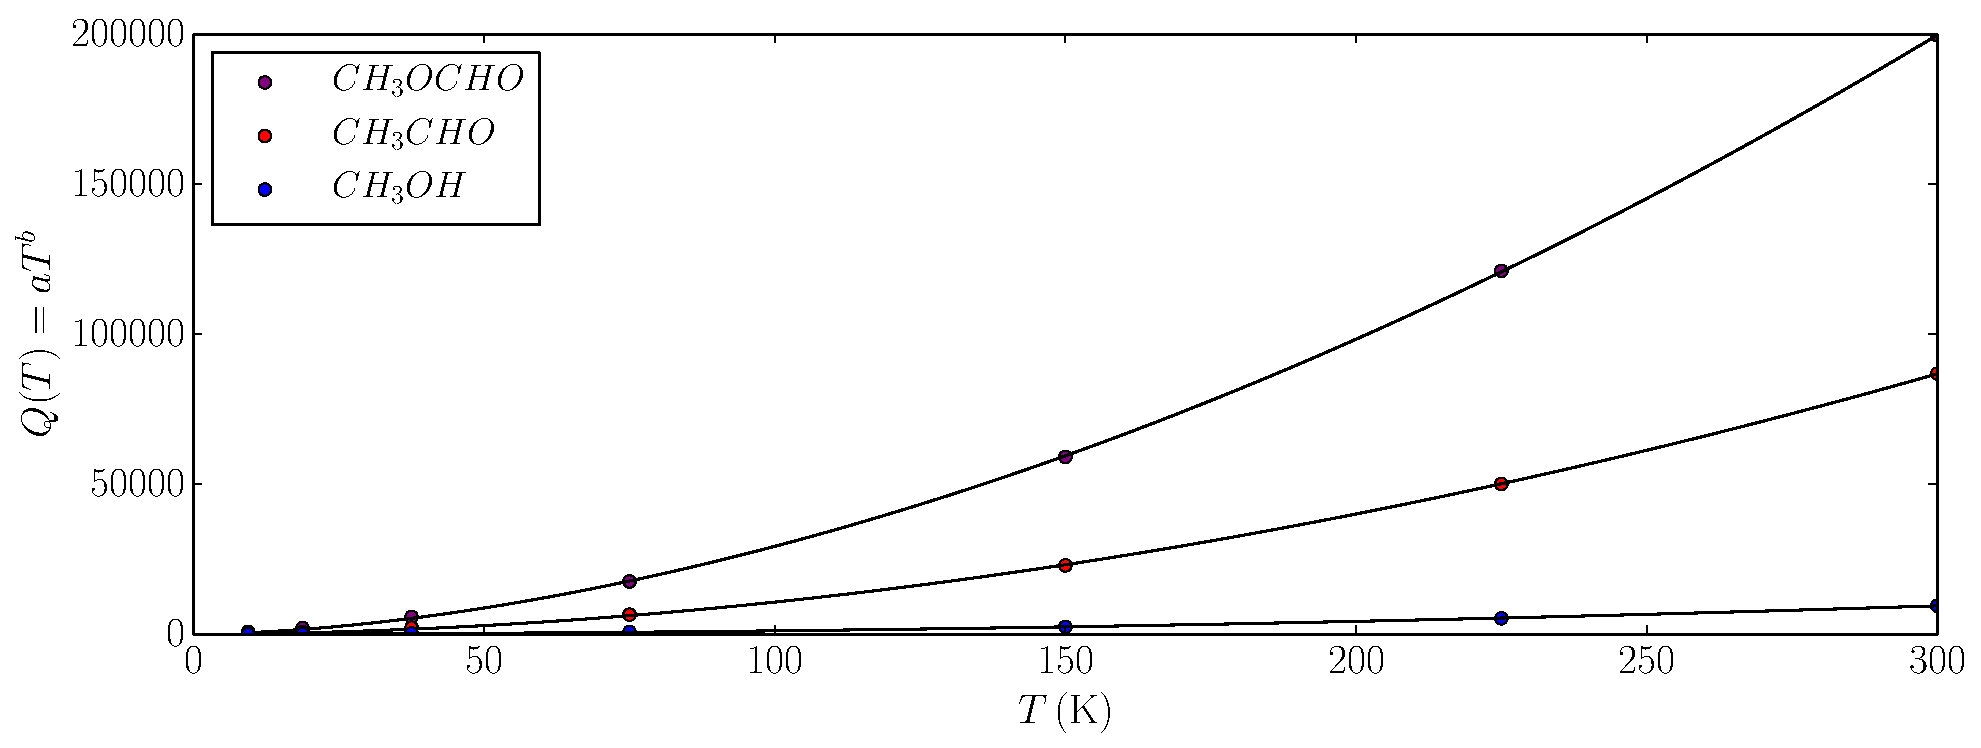
\includegraphics[width=13cm]{PartitionFunction.pdf}
\caption{The partition function data shown with circles for acetaldehyde (red), methanol (blue), and methyl formate (purple) and the corresponding $Q(T) = aT^b$ fit overlaid in black.}
\label{fig:partitionfunction}
\end{center}
\end{figure*}


%%% MOMENT 1 MAPS %%%
\subsubsection{Moment 1 Maps}
\label{subsubsec:mom1}

The first moment (\momone) quantifies the velocity-weighted integrated line intensity, and is calculated by setting $n=1$ in Equation \ref{eq:mom} and normalizing it with the total integrated line intensity,

\begin{align} \label{eq:mom1}
{\mu}_1 = \int_{-\infty}^{\infty} v I(v)dv \Big/ \int_{-\infty}^{\infty} I(v)dv\,.
\end{align}

{\noindent}Discretizing the equation once again, and substituting the known expression for {\momzero} (see Equation \ref{eq:mom0}), the average velocity of the emission line profile is 

\begin{align} \label{eq:avgvel}
<v>{\;}~= \sum_{-\infty}^{\infty} v I(v){\Delta}v \Big/ W\,.
\end{align}

{\noindent}Figure \ref{fig:exmaps} shows an example {\momone} map for a rotational transition of Acetaldehyde in subplot (b). 

\begin{figure}[t]
\begin{center}
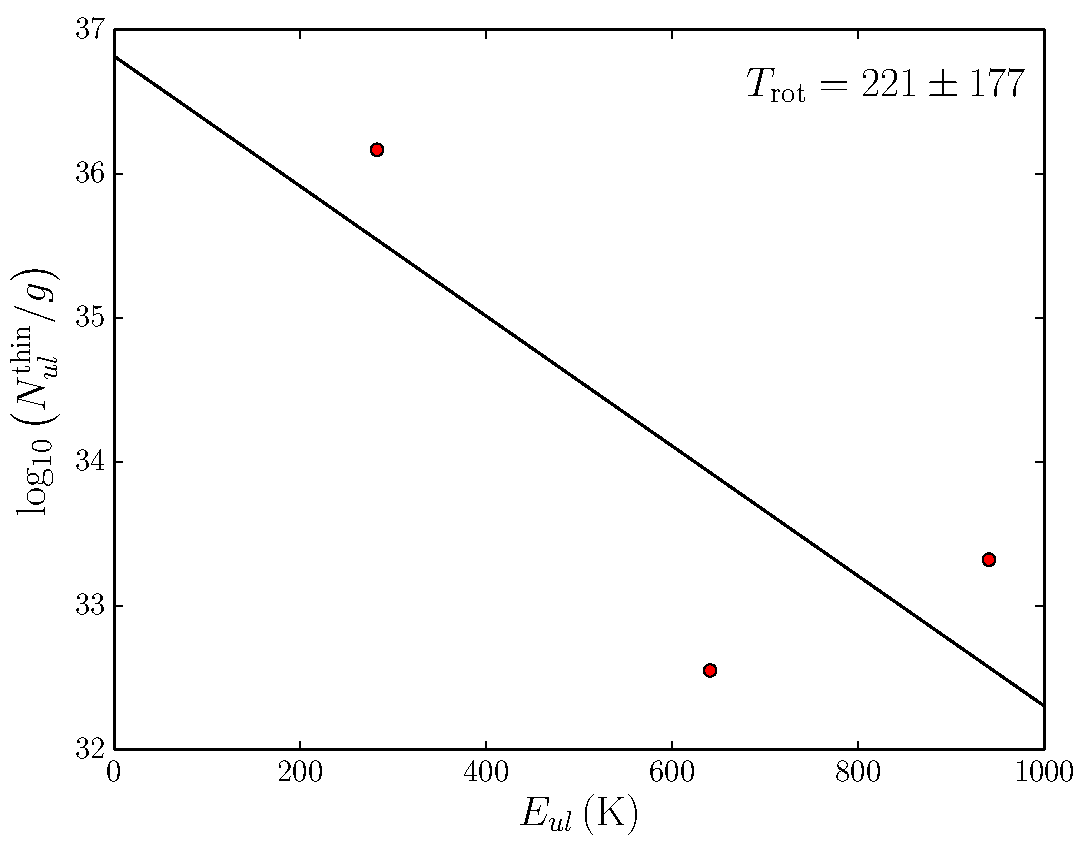
\includegraphics[width=8cm]{PopDiagram.pdf}
\caption{A representative population diagram for acetaldehyde with the fit overlaid that results in {\Trot} = 221 K and {\Ntot} = 4.75 ${\times}10^{20}$ cm$^{-2}$ located at the spatial pixel (132,133). }
\label{fig:PopDiagram}
\end{center}
\end{figure}

%%% MOMENT 2 MAPS %%%
\subsubsection{Moment 2 Maps}
\label{subsubsec:mom2}

The second moment (\momtwo) quantifies the line width or the velocity dispersion of the emission profile, and it calculated by setting $n=2$ in Equation \ref{eq:mom}, and once again, normalizing it with the total integrated line intensity,

\begin{align} \label{eq:mom2}
{\mu}_2 = \sqrt{\frac{\int_{-\infty}^{\infty}I(v)(v-\left[ \int_{-\infty}^{\infty} v I(v)dv \Big/ \int_{-\infty}^{\infty} I(v)dv \right])^2}{\int_{-\infty}^{\infty}I(v)dv}}\,.
\end{align}

{\noindent}Discretizing the equation once more, and substituting the known expressions for {\momzero} (see Equation \ref{eq:mom0}) and {\momone} (see Equation \ref{eq:mom1}), the velocity dispersion is 

\begin{align} \label{eq:dispersion}
<v>^{1/2}{\;}= \sqrt{\frac{\sum_{-\infty}^{\infty}I(v)(v-<v>)^2{\Delta}v}{W}}\,.
\end{align}

{\noindent}Figure \ref{fig:exmaps} shows an example {\momtwo} map for a rotational transition of Acetaldehyde in subplot (c). 

%%% Summary of Partition Functions Table %%%
\begin{deluxetable}{lccccc}
\tablecolumns{5}
\tablecaption{Summary of Partition Functions}
\tablehead{
\multicolumn{3}{c}{} & \colhead{\A} & \colhead{\M} & \colhead{\MF} \T\B\\
\hline
\multicolumn{6}{c}{Data} \T 
} 
\startdata
 & $T$ & & \multicolumn{3}{c}{$Q(T)$} \B\\
\cline{2-2} \cline{4-6}
 & 9.375 &  & 270.1167 & 19.5433 & 720.82 \T\\
 & 18.75 &  & 760.2458 & 68.7464 & 2030.84 \\
 & 37.50 &  & 2154.5221 & 230.2391 & 5772.42 \\
 & 75.0 &  & 6495.8039 & 731.0698 & 17548.82 \\
 & 150.0 &  & 22892.2045 & 2437.7654 & 59072.96 \\
 & 225.0 &  & 50049.7231 & 5267.8635 7 & 121102.02 \\
 & 300.0 &  & 86841.0823 & 9473.1198 & 199602.70 \\
 ref: &  &  & JPL & JPL & CDMS \B\\
 \hline
\multicolumn{6}{c}{$Q(T)=aT^b$ Fit Parameters} \T\B\\
\hline
  & a & & 1.6 $\pm$ 0.1 & 0.13 $\pm$ 0.03 & 9.3 $\pm$ 0.4 \T\\
  & b & & 1.91 $\pm$ 0.02 & 1.96 $\pm$ 0.04 & 1.748 $\pm$ 0.007
\enddata
\label{table:partitionfunction}
\end{deluxetable}

%%% POPULATION DIAGRAM %%%
\subsection{Population Diagram}
\label{subsec:popdiagram}

If the molecular emission is optically thin and in local thermodynamic equilibrium (LTE), the total column density of a molecular species can be expressed as

\begin{align}
N_{tot} = \frac{N_{ul}^\mathrm{thin}}{Q(T)}\,g_{ul}\,e^{-E_{ul}/kT_\mathrm{rot}} \, ,
\end{align}

{\noindent}where all excitation temperatures are equal and are coupled with the gas kinetic temperature. 

\begin{figure*}[t]
\begin{center}
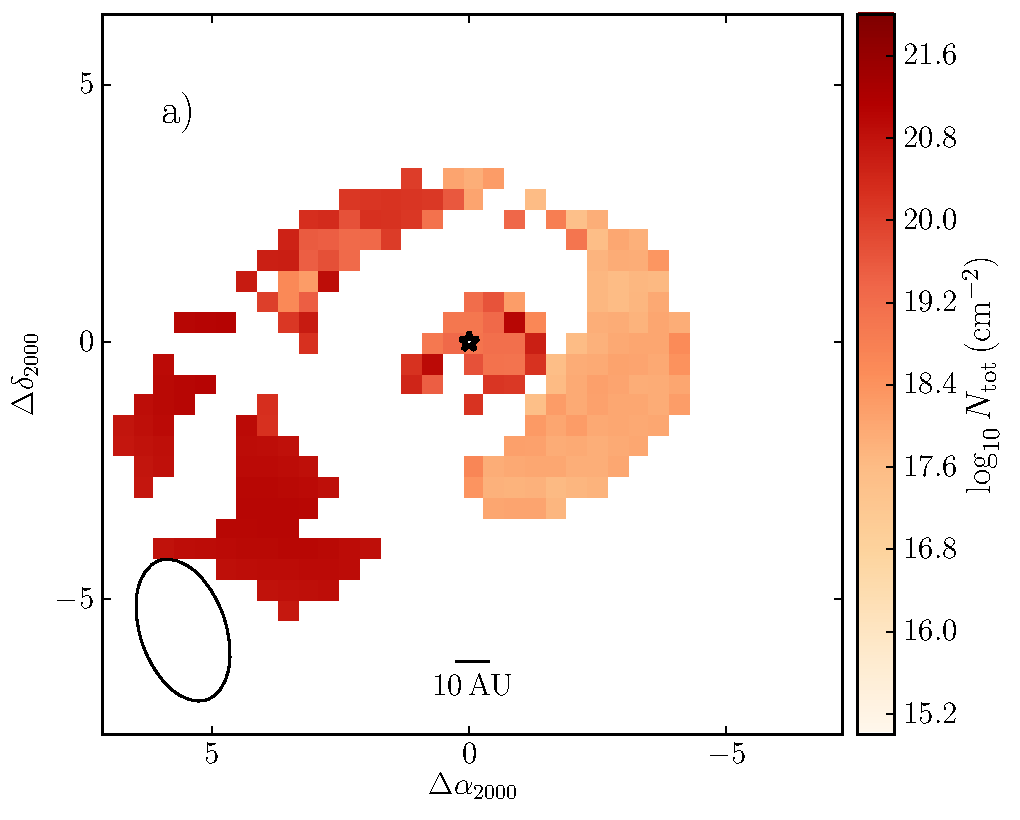
\includegraphics[width=5.95cm]{Acetaldehyde_Nmap.pdf} 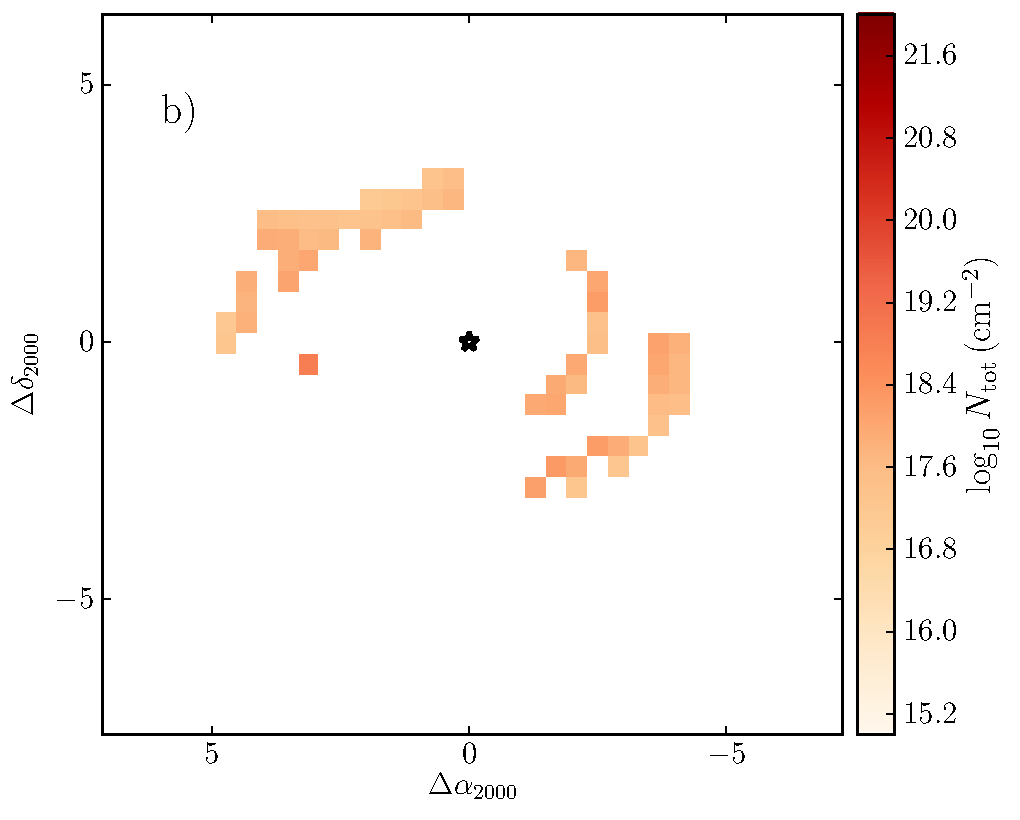
\includegraphics[width=5.95cm]{Methanol_Nmap.pdf} 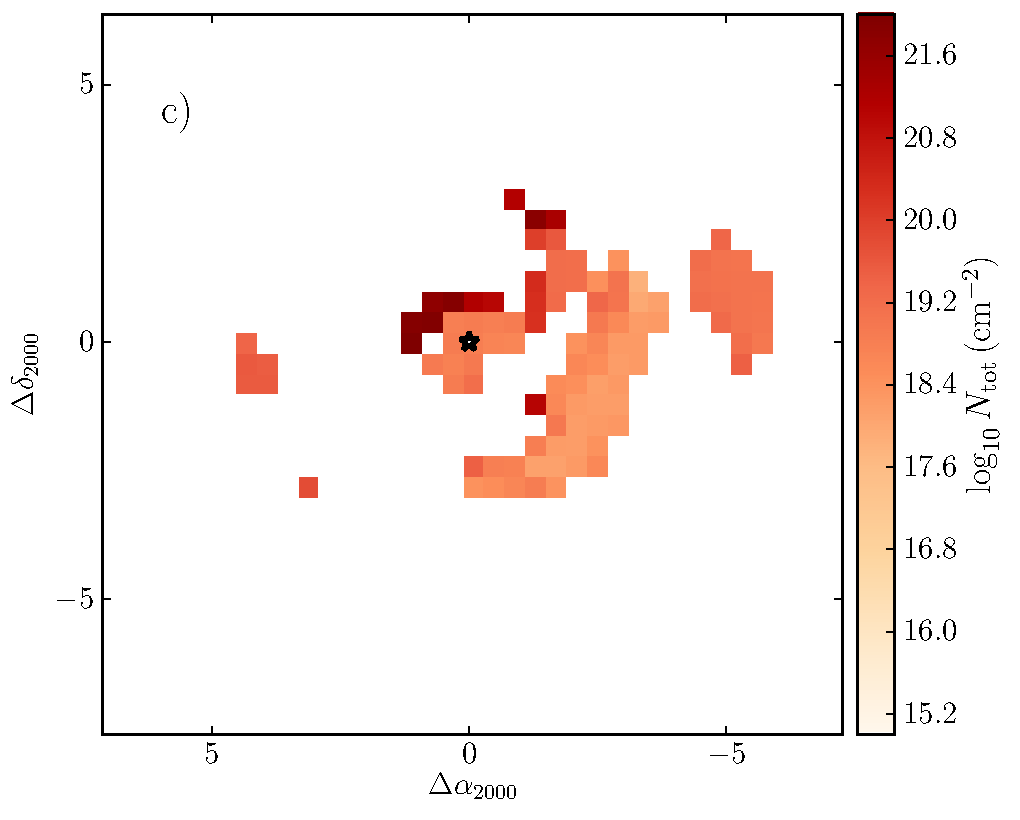
\includegraphics[width=5.95cm]{MethylFormate_Nmap.pdf}
\caption{Total column density (\Ntot) maps for (a) acetaldehyde, (b) methanol, and (c) methyl formate. The (black) star symbol indicates the pointing position of the IRAS B protostar and the approximate ALMA beam is shown in the bottom left corner. The spatial regions of the map are shown for those where $0.0 \, \mathrm{K} < T_\mathrm{rot} < 2500 \, \mathrm{K}$ and correspond to the same regions shown in Figure \ref{fig:Tmaps} (above).}
\label{fig:Nmaps}
\end{center}
\end{figure*}

\begin{figure*}[t]
\begin{center}
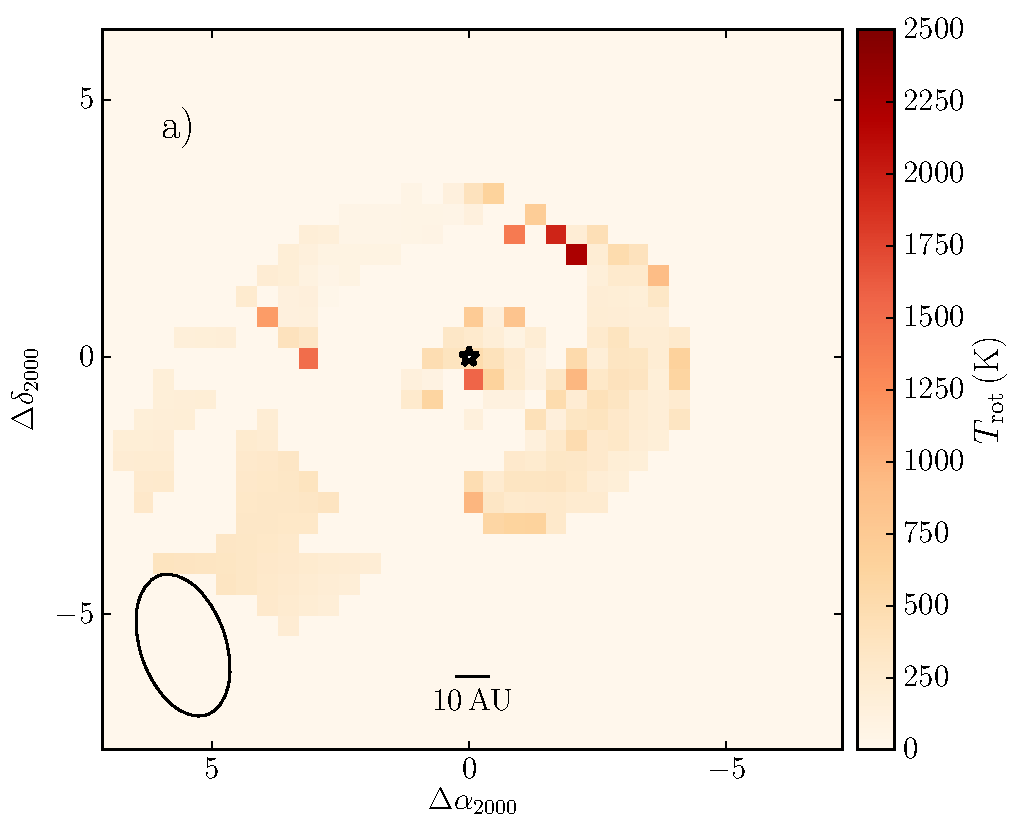
\includegraphics[width=5.95cm]{Acetaldehyde_Tmap.pdf} 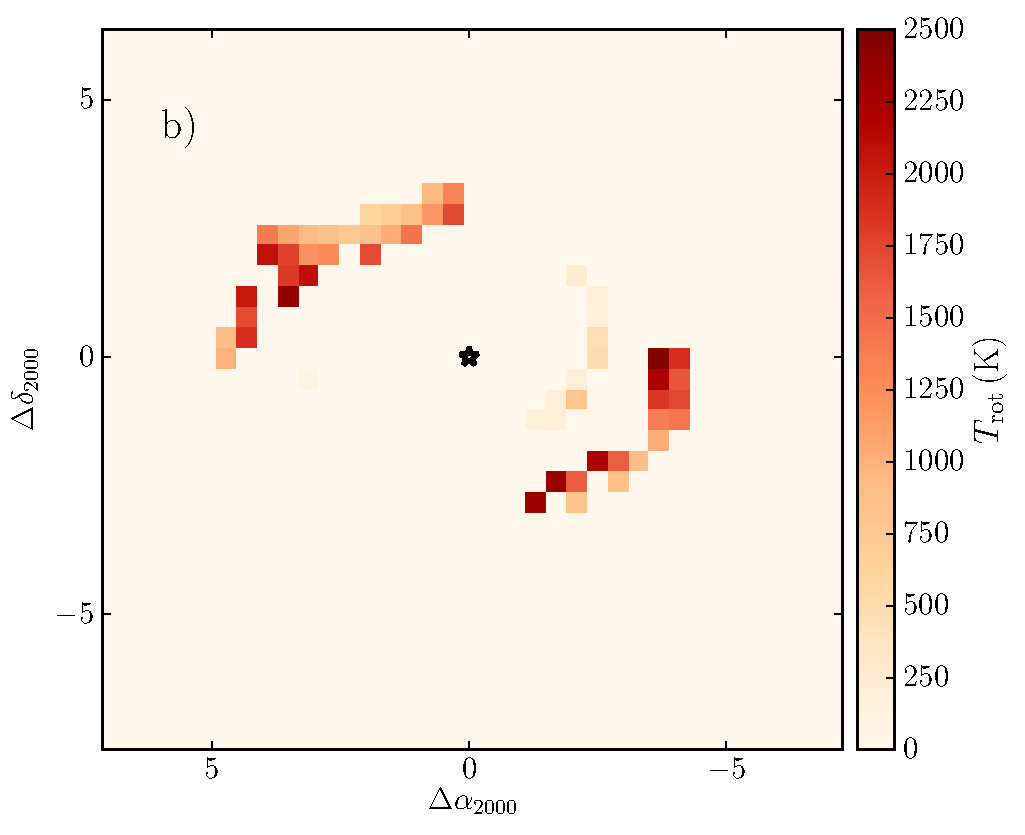
\includegraphics[width=5.95cm]{Methanol_Tmap.pdf} 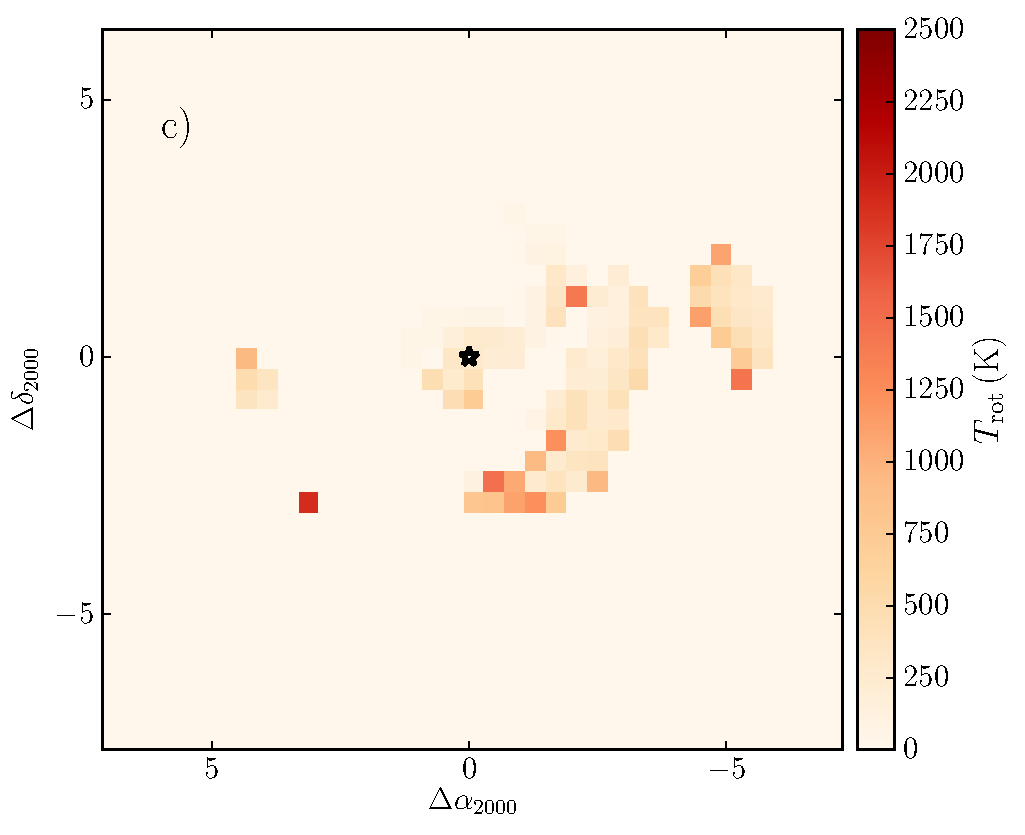
\includegraphics[width=5.95cm]{MethylFormate_Tmap.pdf}
\caption{Rotational temperature (\Trot) maps for (a) acetaldehyde, (b) methanol, and (c) methyl formate. The (black) star symbol indicates the pointing position of the IRAS B protostar and the approximate ALMA beam is shown in the bottom left corner. The spatial regions of the map are shown for those where $0.0 \, \mathrm{K} < T_\mathrm{rot} < 2500 \, \mathrm{K}$.}
\label{fig:Tmaps}
\end{center}
\end{figure*}

A popular technique for analyzing molecular cloud gas properties is the ``population diagram'', also called the ``rotational diagram'' \citep[e.g.,][]{Bisschop2008}. With detections of multiple molecular transitions that span a range in excitation energies, this method consists of plotting the natural logarithm of the column density per statistical weight of each molecular energy level as a function of their upper-level energy. If the gas is optically thin and in local thermodynamic equilibrium (LTE), this will be a Boltzmann distribution. Thus, a plot of the natural logarithm of {\Nthin}/$g$ as a function of {\Eul} will yield a straight line whose slope is related to the rotational (excitation) temperature (\Trot) and whose y-intercept is related to the total column density of the molecular species ({\Ntot}). Fitting a line representing the function

\begin{align} \label{eq:popdiagram}
ln \left( \frac{N_{ul}^\mathrm{thin}}{g} \right) = ln \left( \frac{N_{\mathrm{tot}}}{Z(T_\mathrm{rot})} \right) - \left( \frac{E_{ul}}{k} \right) \frac{1}{T_\mathrm{rot}}
\end{align}

{\noindent}allows for a direct measure of these quantities. The partition function, $Q(T)$, was determined by fitting the function $Q(T) = aT^b$ to publicly available partition function data from the JPL and CDMS catalogs using the Python Scipy {\tt curve\_fit} routine\footnote{\url{http://www.scipy.org/}} (used hereafter for all fitting procedures). With detections having temperatures of up to $\sim$\,2,500\,K, this fit assumes that the partition function exhibits the same behaviour beyond 300\,K. A more in-depth routine might include calculating the partition function rather than fitting it for $0\,K < T < 300\,K$ and extrapolating it to 2,500\,K. Table \ref{table:partitionfunction} summarizes the partition function details, including the data used and the fitting results. Figure \ref{fig:partitionfunction} shows the partition function fit obtained for acetaldehyde (red), methanol (blue), and methyl formate (purple), with the fit overlaid (black).

To use the population diagram technique for determining rotational temperatures and total molecular column densities, the column densities of each upper-level energy transition were first calculated following

\begin{align}
N_{ul}^\mathrm{thin} = \frac{W 4{\pi}d^2}{10^{26}hcA_{ul}{\Omega}}\,.
\end{align}

{\noindent}Here, $W$ is the integrated line intensity in {\Jybeamkms} (see Equation \ref{eq:W}), $d$ is the distance to the source in parsecs, {\Aul} is the upper-level Einstein A coefficient, and $\Omega$ is the beam area in cm$^2$ which can be calculated using the major and minor axes of the beam size (${\theta}_\mathrm{maj}$ and ${\theta}_\mathrm{min}$, respectively) as

\begin{align}
\Omega = \frac{{\pi}{\theta}_\mathrm{min}{\theta}_\mathrm{maj}}{4log2}\,.
\end{align}

{\noindent}Figure \ref{fig:exmaps} shows an example {\Nthin} map for a rotational transition of Acetaldehyde in subplot (d). 

The total column density (\Ntot) of the molecular species were then determined by applying a fit to Equation \ref{eq:popdiagram} and calculating the y-intercept. Figure \ref{fig:Nmaps} shows the resulting {\Ntot} maps of (a) acetaldehyde, (b) methanol, and (c) methyl formate. The same fit was used to determine the rotational temperature (\Trot) of the molecular species by calculating the inverse of the slope. Figure \ref{fig:Tmaps} shows the resulting {\Trot} maps of (a) acetaldehyde, (b) methanol, and (c) methyl formate. The regions where the population diagram technique was applied are those where there were at least two 5\,$\sigma$ detections of rotational transitions in $W$ with upper-level energies separated by at least 50 K to ensure that Equation \ref{eq:popdiagram} could be fit (i.e., you cannot fit a line to a single point). The {\Trot} and {\Ntot} maps are restricted to regions satisfying $0.0 \, \mathrm{K} < T_\mathrm{rot} < 2500 \, \mathrm{K}$ (this is discussed in more detail in Section \ref{subsec:coltempmaps}).

\begin{figure}[t]
\begin{center}
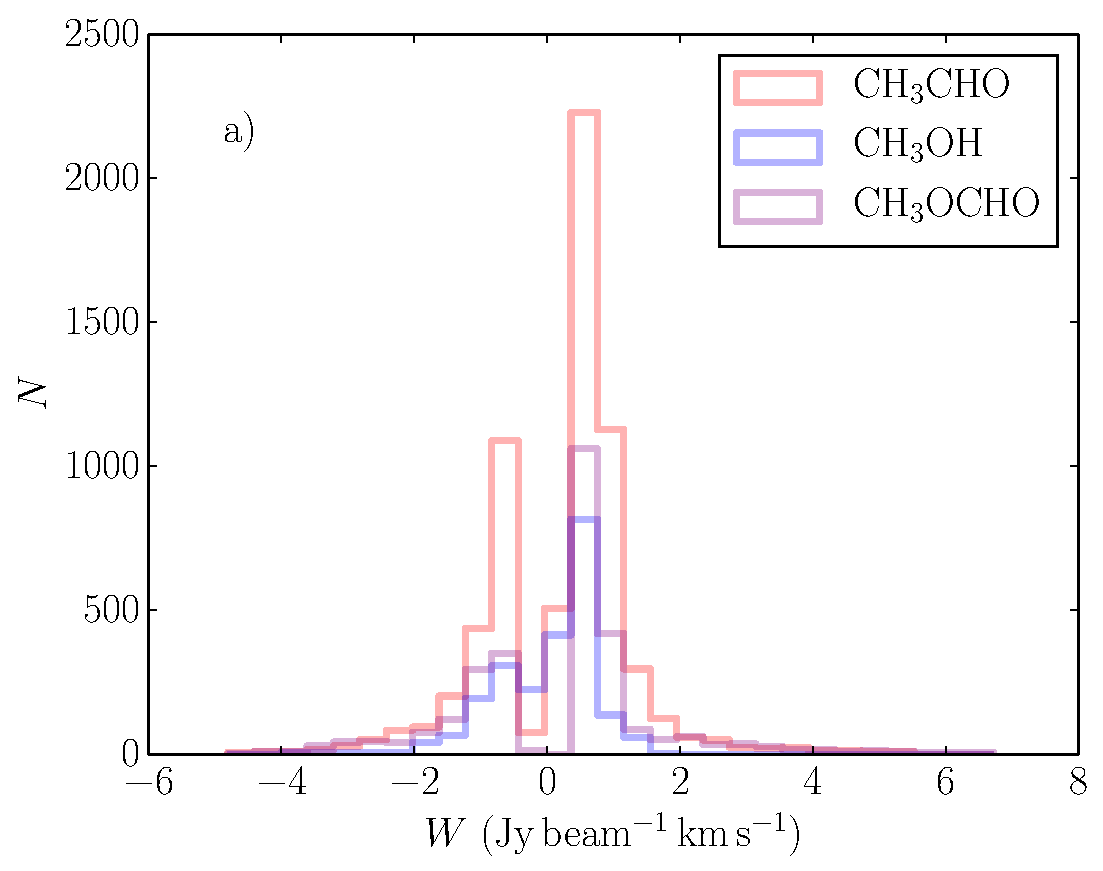
\includegraphics[width=8cm]{mom0_hist.pdf}

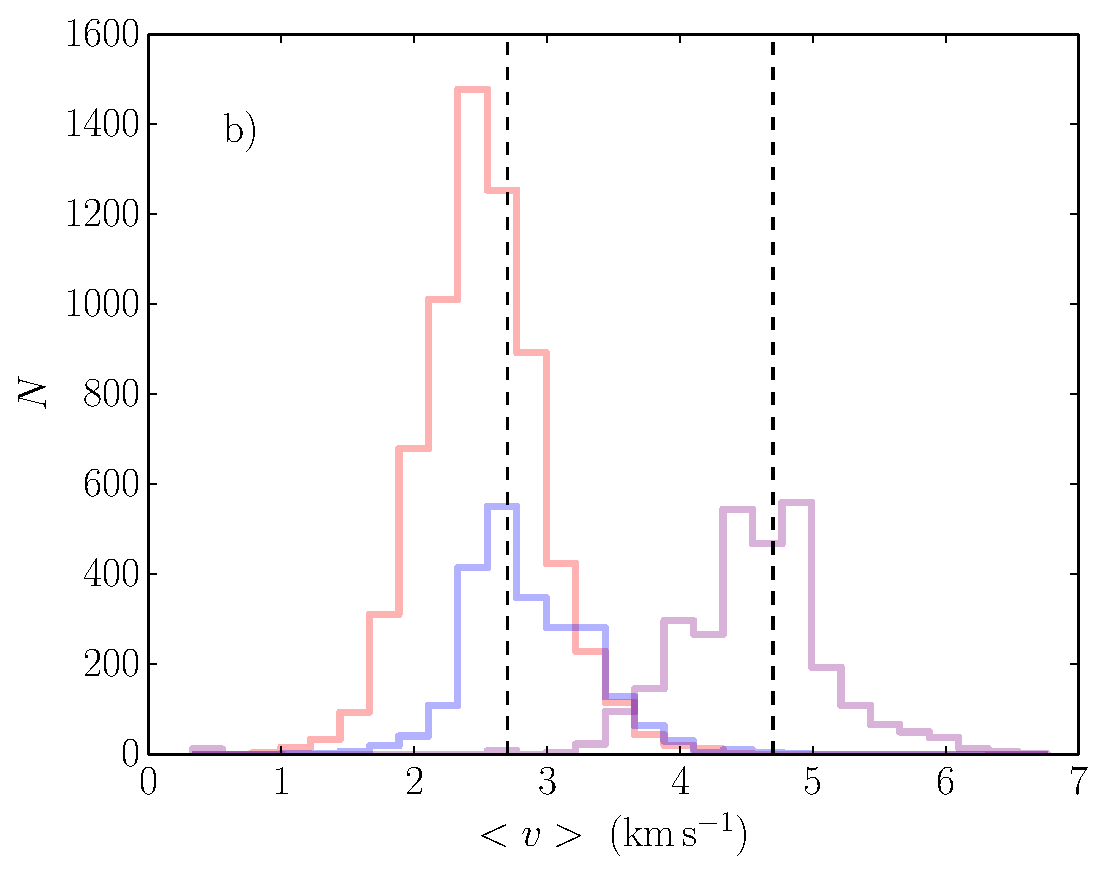
\includegraphics[width=8cm]{mom1_hist.pdf}

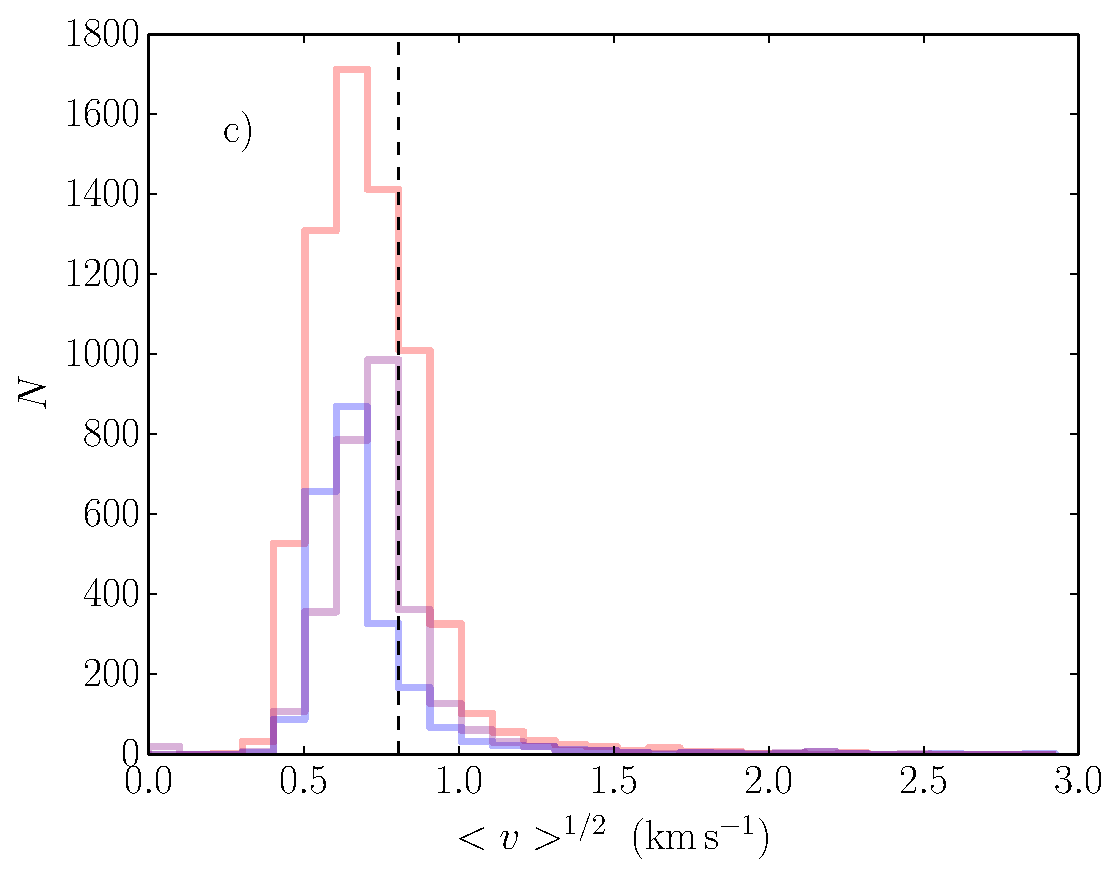
\includegraphics[width=8cm]{mom2_hist.pdf}
\caption{Distributions of (a) $W$, (b) $<v>$, and (c) $<v>^{1/2}$, corresponding to {\momzero}, {\momone}, and {\momtwo} moment maps, respectively. Acetaldehyde is shown in red, methanol is shown in blue, and methyl formate is shown in purple.}
\label{fig:momenthist}
\end{center}
\end{figure}

\begin{figure}
\begin{center}
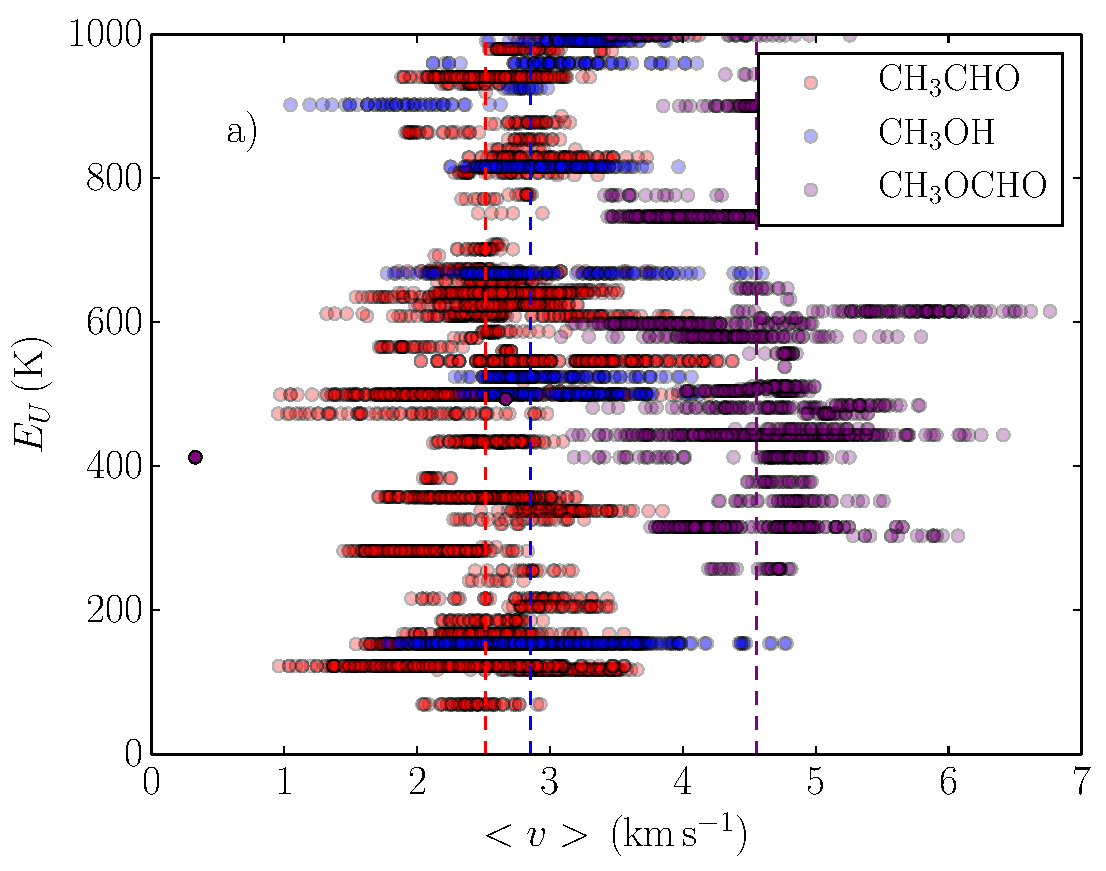
\includegraphics[width=8cm]{Energy_mom1.pdf} 

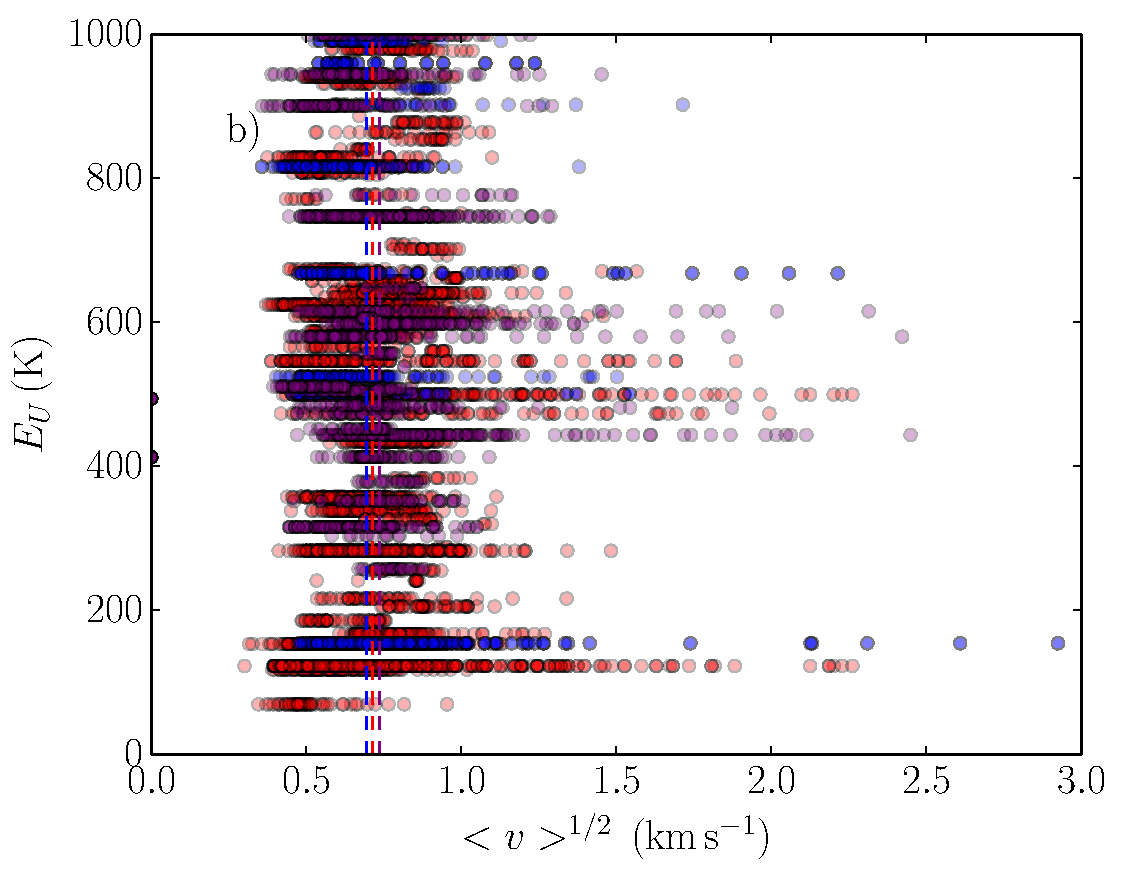
\includegraphics[width=8cm]{Energy_mom2.pdf} 

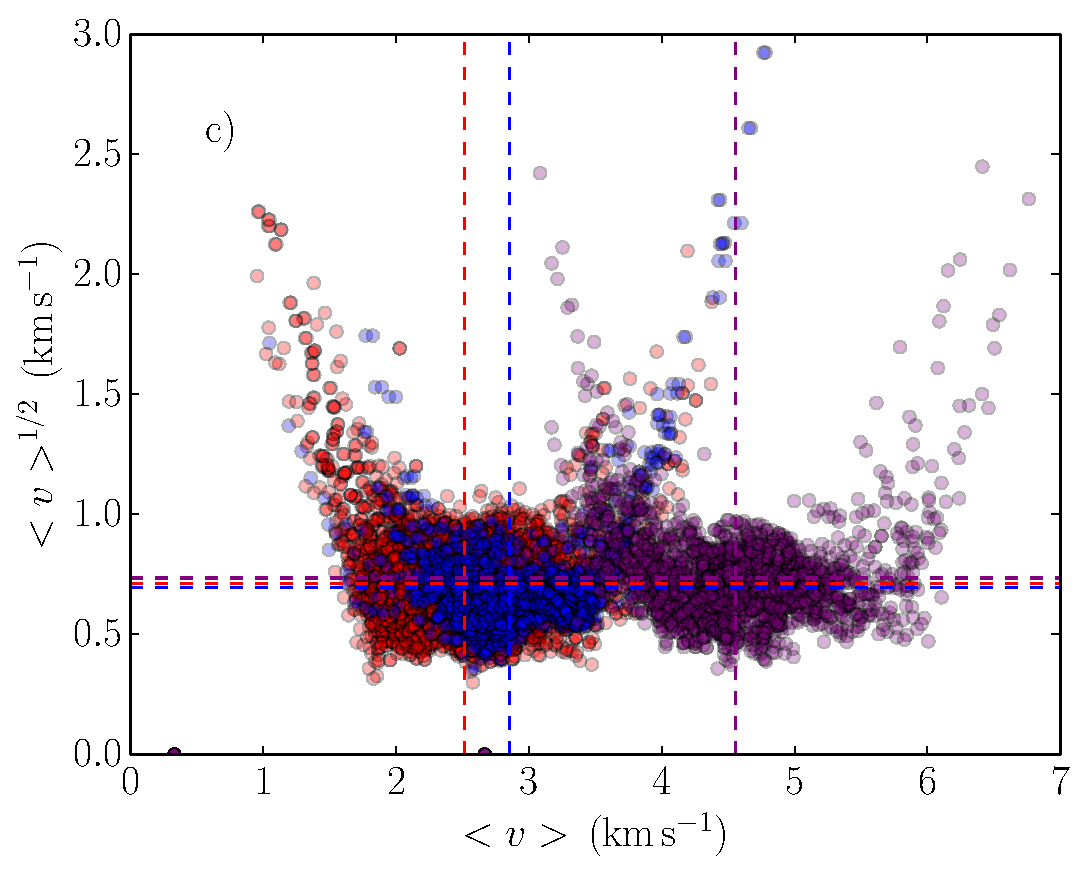
\includegraphics[width=8cm]{mom2_mom1.pdf}
\caption{Correlation plots of (a) upper-level energy versus velocity, (b) upper-level energy versus velocity dispersion, and (c) velocity dispersion velocity velocity for all 5\,$\sigma$ detections. Acetaldehyde is shown in red, methanol in blue, and methyl formate in purple.}
\label{fig:correlations}
\end{center}
\end{figure}

%%% DISCUSSION %%% 
\section{Discussion}
\label{sec:discussion}

Here we discuss the results of IRAS 1624 that were analyzed using the Python pipeline, starting with the moment maps, followed by the {\Ntot} and {\Trot} maps, and finishing with future work. 

\subsection{Moment Maps}
\label{subsec:mommaps}

In this section, we will discuss the $W$, $<v>$, and $<v>^{1/2}$ maps which correspond to the {\momzero}, {\momone}, and {\momtwo} moment maps, respectively. Results in this section are from all detections above the 5\,$\sigma$ level in $W$ at each spatial pixel for all rotational transitions of each molecule. For acetaldehyde, this corresponds to 6,619 detections, for methanol 2,301 detections, and for methyl formate 2,904 detections. 

The distributions in $W$ are very similar for all three molecules. The median values for emission are 0.67 {\Jybeamkms}, 0.47 {\Jybeamkms}, and 0.69 {\Jybeamkms} for acetaldehyde, methanol, and methyl formate, respectively. The median values for absorption are $-0.76$ {\Jybeamkms}, $-0.70$ {\Jybeamkms}, and $-1.01$ {\Jybeamkms} for acetaldehyde, methanol, and methyl formate, respectively. Values in $W$ are found to be as low as $-4.81$ {\Jybeamkms} and as high as 6.72 {\Jybeamkms}, which are likely being affected by blending with crowded emission lines. The distributions of $W$ are shown at the top of Figure \ref{fig:momenthist}. 

As discussed in Section \ref{subsec:detections}, both acetaldehyde and methanol were found at a source velocity of {\vLSR} = 2.7 \kms, while methyl formate was located at {\vLSR} = 4.7 \kms. Acetaldehyde and methanol, therefore, have similar $<v>$ distributions which themselves are different than that of methyl formate. Acetaldehyde is found to have a median source velocity of 2.5 \kms, while methanol has a median source velocity of 2.8 \kms. Methyl formate, on the other hand, has a medium source velocity located at 4.6 \kms. Acetaldehyde and methanol also exhibit similar standard deviations of these distributions, 0.45 {\kms} and 0.46 \kms, respectively, while methyl formate has a higher standard deviation of 0.60 \kms. It seems therefore that acetaldehyde and methanol have similar {\vLSR} distributions while methyl formate is comparatively quite different. The distributions of $<v>$ are shown in the middle of Figure \ref{fig:momenthist}. It seems likely that these features are the result of line-blending. A closer look at these features is required.

Despite the differences in the distributions of $<v>$, the distributions in $<v>^{1/2}$ are quite similar across the three molecules. Acetaldehyde, methanol, and methyl formate have median $<v>^{1/2}$ values of 0.69 \kms, 0.65 \kms, and 0.72 \kms, with standard deviations of 0.19 \kms, 0.21 \kms, 0.19 \kms, respectively. While methyl formate's difference in $<v>$ seems significant (see above), the similarities in $<v>^{1/2}$ raises the question of how different the kinematics really are. A more detailed analysis on the source velocities of the molecules are required (e.g., more rigorous LTE modeling) to strengthen these findings. The distributions in $<v>^{1/2}$ are shown in the bottom of Figure \ref{fig:momenthist}.

We also investigate the relationship between {\vLSR} and {\dispersion} (using their respective moment maps) and the upper-level energy of the transition, as well as the relationship between themselves. Similar to the findings of \citet{Jorgensen2011}, we find no trend of {\vLSR} nor {\dispersion} with the {\Eul}, shown in the top and middle of Figure \ref{fig:correlations}, respectively. A plot of {\dispersion} versus {\vLSR} however, shown in the bottom of Figure \ref{fig:correlations}, shows an interesting structure whereby a positive correlation is seen for $v > v_\mathrm{LSR}$ and an anti-correlation is seen for $v < v_\mathrm{LSR}$ for each of the three molecules. These features are likely the result of line blending. A possibility to test this may be to decrease/increase the frequency range that defines each emission line to see if these features weaken/strengthen.

\subsection{Column Density Maps and Rotational Temperature Maps}
\label{subsec:coltempmaps}

The acetaldehyde, methanol, and methyl formate rotational transitions span a wide range of column densities (\Nthin). Column densities are found as low as $10^{12.3}$\,cm$^{-2}$ and as high as $10^{19.0}$\,cm$^{-2}$, which is almost seven orders of magnitude. Acetaldehyde and methanol alone are found to trace gas that spans 5.5 and 5.8 orders of magnitude in column density, while methyl formate spans 3.5 orders of magnitude. Acetaldehyde and methyl formate have median {\Nthin} values of $10^{14.4}$\,cm$^{-2}$ and $10^{15.3}$\,cm$^{-2}$, respectively, while methanol has a lower median {\Nthin} value of $10^{13.5}$\,cm$^{-2}$. 

Figure \ref{fig:Nmaps} shows the {\Ntot} maps for (a) acetaldehyde, (b) methanol, and (c) methyl formate. Section \ref{subsec:popdiagram} discusses how the regions with detections were determined. It is clear that the three molecules are tracing gas in different spatial regions of IRAS B. While acetaldehyde and methyl formate have somewhat extended emission, methanol seems to trace more compact emission. This could, however, be due to the comparatively lower number of detections in methanol (18) than acetaldehyde (97) and methyl formate (50). The total column density of the molecules (\Ntot) ranges from $10^{17.1}$\,cm$^{-2}$ to $10^{22.3}$\,cm$^{-2}$, which is approximately 5 orders of magnitude. Acetaldehyde and methyl formate spans 3.6 and 4.5 orders of magnitude, respectively, while methanol spans 1.7 orders of magnitude in \Ntot. Acetaldehyde is found to have a median {\Ntot} value of $10^{19.3}$\,cm$^{-2}$, with $10^{17.7}$\,cm$^{-2}$ and $10^{18.9}$\,cm$^{-2}$ for methanol and methyl formate, respectively. The observed column densities are quite high, and further investigation is required to better understand what may be causing these values to be so unusually high. While they are likely being affected by line blending, which is a significant obstacle with the extent of line crowding present in the data and requires more careful investigation and correction, this effect is unlikely to cause column densities several orders of magnitude higher than expected.

Figure \ref{fig:Tmaps} shows the {\Trot} maps for (a) acetaldehyde, (b) methanol, and (c) methyl formate. Rotational temperatures (\Trot) are found between 23\,K and 2,451\,K. In addition to each of the three molecules tracing gas with a range of column densities, there also is a wide range of rotational temperatures present. Acetaldehyde traces gas from 23\,K to 2,228\,K, while methanol traces gas from 94\,K to 2,451\,K and methyl formate from 49\,K to 1,898\,K. Acetaldehyde is found to trace a median {\Trot} of 254\,K, with a median value of 1,189\,K for methanol and 307\,K for methyl formate. While the {\Trot} found for acetaldehyde is consistent with a previous combined JCMT and IRAM survey \citep{Caux2011}, further investigation on the large uncertainties in {\Trot} are required. While many spatial pixels result in ``reasonable'' {\Trot} values (see Figure \ref{fig:Tmaps}), there still remain many regions with unphysical (i.e., negative) temperatures or large uncertainties. Using the quantum numbers to focus on specific K-ladders may help to elucidate this.

\begin{figure}[t]
\begin{center}
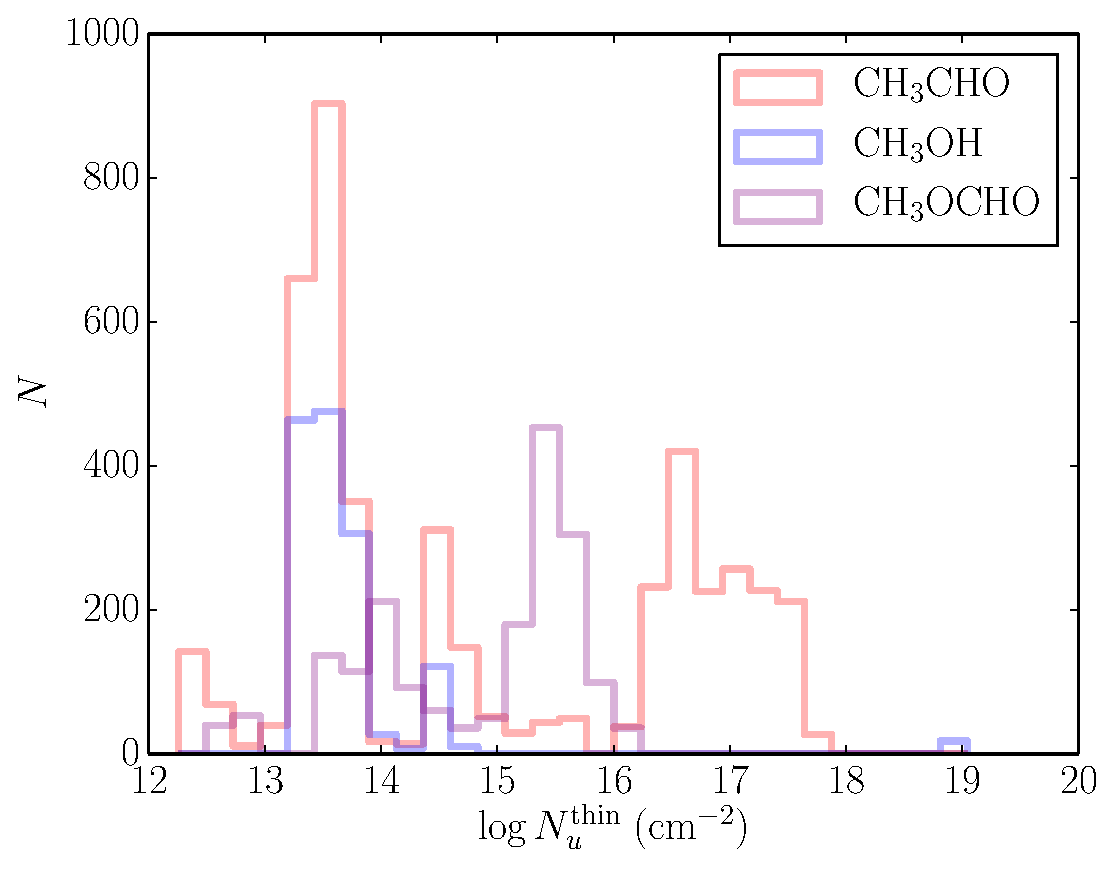
\includegraphics[width=8cm]{Nthin_hist.pdf}

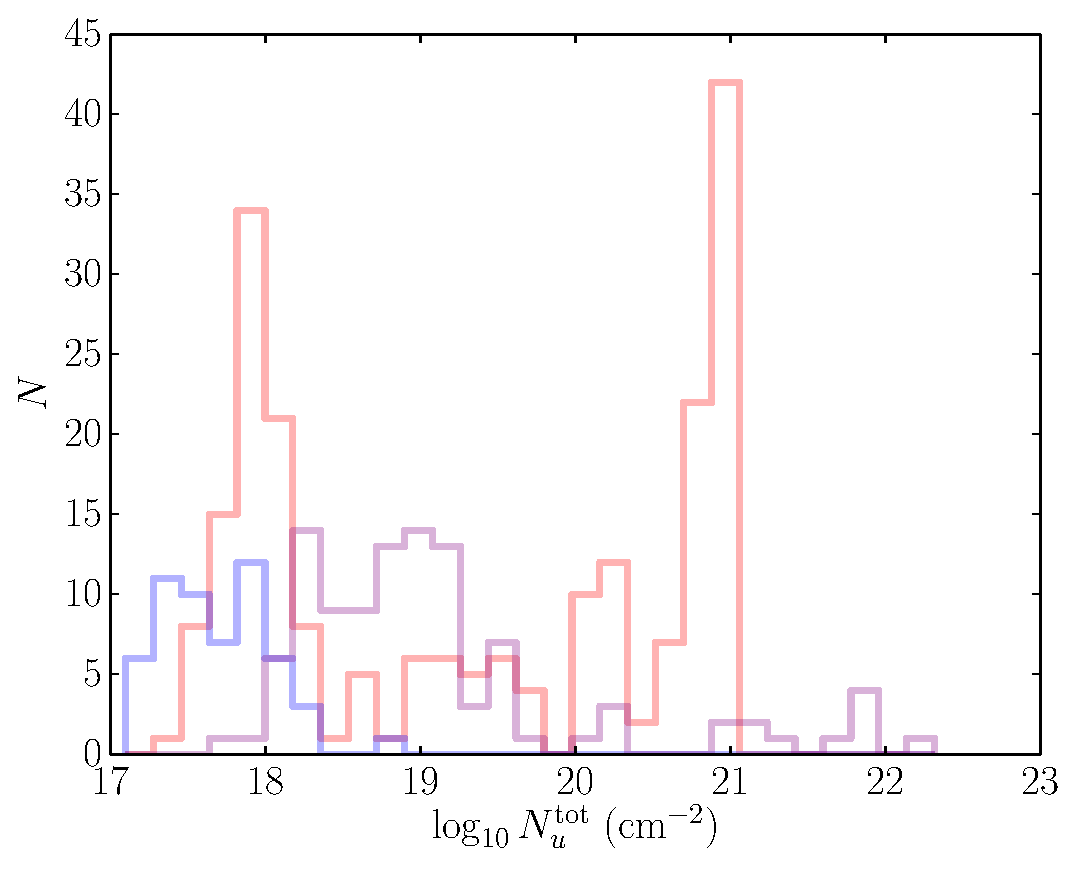
\includegraphics[width=8cm]{Ntot_hist.pdf}

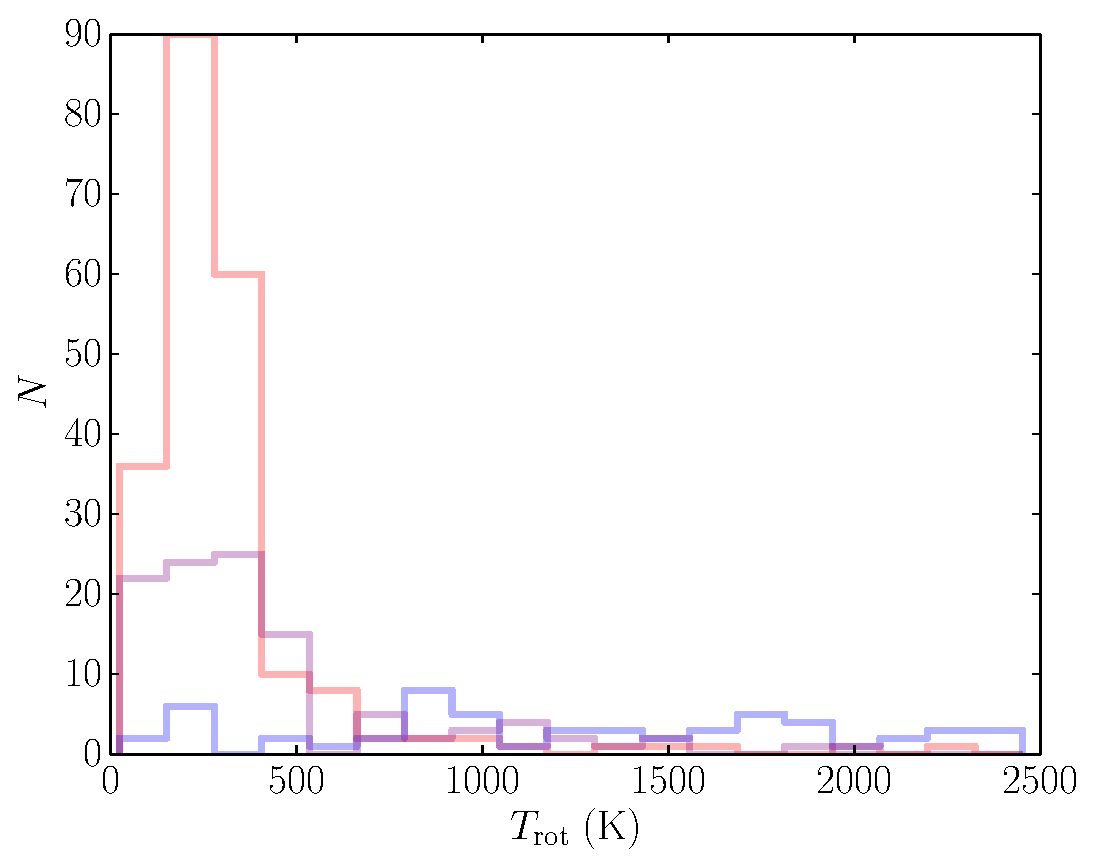
\includegraphics[width=8cm]{Trot_hist.pdf}
\caption{Distributions of (a) $W$, (b) $<v>$, and (c) $<v>^{1/2}$, corresponding to {\momzero}, {\momone}, and {\momtwo} moment maps, respectively. Acetaldehyde is shown in red, methanol is shown in blue, and methyl formate is shown in purple.}
\label{fig:tempdenhist}
\end{center}
\end{figure}

\subsection{Future Work}

The following are aspects of the pipeline that serve to be improvements in the future:

\begin{itemize}

\item Scanning all spectral baselines to measure the median sensitivity of each spatial pixel for more accurate noise maps.
\item Calculating the partition function directly instead of fitting and interpolating to high temperature values.
\item Implementing an automated way to correct for line blending.
\item Creating population diagrams for specific K quantum numbers which may help to shed light on the non-physical temperatures and high uncertainties in the current pipeline. Understanding the format of the quantum numbers provided by the JPL and CDMS databases will be required (some have 2 or 3 quantum numbers instead of 4 and need to be separated properly).
\item Investigate the (anti-) correlation seen in the {\dispersion} versus {\vLSR} plot by increasing the frequency/velocity range of the spectral window used for the measurements of each emission line. If these (anti-) correlations strengthen (or weaken if the frequency range is decreased), these features are then likely the result of line blending.
\end{itemize}

%%% SUMMARY %%%
\section{Summary}
\label{sec:summary}

We construct a Python pipeline to analyse the high quality, spatially resolved ALMA data of the deeply-embedded low-mass protostar {\IRAS}. In summary, the steps that the Python pipeline performs are the following:

\begin{itemize}
\item Molecular lines were identified for pure rotational transitions present in the frequency ranges of each spw using the JPL and CDMS catalogs. Splatalogue was not used to query these database since several emission lines were missing.
\item Descriptors of the transition were obtained including the rest frequency (\restfreq) of the transition, resolved quantum numbers of the transition, Einstein A coefficient of the upper-level (\Aul), the upper-level energy (\Eul), and the statistical weight of the upper level ($g_{ul}$).
\item Noise maps were made using pre-defined frequency ranges specific for each spw.
\item Using a source velocity (\vLSR) and velocity dispersion ($\sigma$) of the source, a spectral slab that is 1.5\,$\sigma$ about the source {\vLSR} was obtained. We determine a source local standard-of-rest velocity of {\vLSR} = 2.7 {\kms} for acetaldehyde and methanol, and {\vLSR} = 4.7 {\kms} for methyl formate, using LTE modeling.
\item The {\momzero}, {\momone}, and {\momtwo} moment maps were calculated, corresponding to $W$, $<v>$, and $<v>^{1/2}$ maps, respectively. These maps were calculated by ``brute force'', but the $W$ map was also calculated using {\tt spectral-cube} to investigate the residual variance between the two as a sanity check. 
\item Line blending was identified by eye and corrected using the {\Aul} and $g_{ul}$ of each transition.
\item The spatial pixel with the strongest $W$ detection was used to visualize a spectrum representative for each detected transition. 
\item The column densities of each transition (\Nthin) were calculated using the $W$ maps. 
\item The three moment maps ({\momzero}, {\momone}, {\momtwo}), the column density maps (\Nthin), and noise maps were saved to a FITS file for each transition. The spectrum corresponding to the strongest $W$ detection was also saved to a FITS file for each transition (if applicable). Any useful information related to the transition and the source were added to the FITS header.
\item Histograms of the three moment maps as well as column densities for all detections of rotational transitions above a 5\,$\sigma$ level were made.
\item Correlation plots of {\vLSR} and {\dispersion} versus {\Eul} as {\vLSR} versus {\dispersion} were made.
\item Histograms of total column densities and rotational temperatures of the three molecules were made for spatial regions satisfying $0\,\mathrm{K} < T_\mathrm{rot} < 2,500\,\mathrm{K}$ were made.
\end{itemize}

The following summarizes the results: 

\begin{enumerate}

\item Using an LTE model, acetaldehyde and methanol were found to be located at a local standard-of-rest velocity of {\vLSR} = 2.7 \kms, while methyl formate is located at {\vLSR} = 4.7 \kms.
\item We detect 97/220 (44\%) acetaldehyde, 18/32 (56\%) methanol, and 50/116 (43\%) methyl formate pure rotational transitions in IRAS B above the 5\,$\sigma$ level. 
\item The excitation energies detected with acetaldehyde range from 69.48\,K to 998.81\,K, methanol from 154.25\,K to 990.87\,K, and methyl formate from 257.75\,K to 998.82\,K.
\item Assuming a model for the partition function of $Q(T) = aT^b$, we determine $(1.6\pm0.1)T^{1.91\pm0.02}$ for acetaldehyde, $(0.13\pm0.03)T^{1.96\pm0.04}$ for methanol, and $(9.3\pm0.4)T^{1.748\pm0.007}$ for methyl formate. 
\item While acetaldehyde and methyl formate have somewhat extended emission, methanol is found to be more compact. This may however be due to the lower number of detections in methanol.
\item Despite the differences in the distributions of {\vLSR}, all three molecules have very similar distributions in {\dispersion}. Acetaldehyde, methanol, and methyl formate have median {\vLSR} values of 2.5 \kms, 2.8 {\kms}, 4.6 \kms, respectively. Acetaldehyde, methanol, and methyl formate have median $<v>^{1/2}$ values of 0.69 \kms, 0.65 \kms, and 0.72 \kms, with standard deviations of 0.19 \kms, 0.21 \kms, 0.19 \kms, respectively.
\item We find no correlation between {\Eul} and {\vLSR} nor {\Eul} and {\dispersion}.
\item We find a correlation between {\dispersion} and {\vLSR} for $v > v_\mathrm{LSR}$ and an anti-correlation for $v < v_\mathrm{LSR}$ that is likely the result of line blending. 
\item The total column densities {\Ntot} found were higher than those in previous studies. Line blending and ALMA's comparatively small beam size do not alone explain the high {\Ntot} found in this analysis, and requires further investigation. 
\item Acetaldehyde was found to have a median {\Trot} of 254\,K, which is consistent is previous studies. Methanol and methyl formate were found to have median {\Trot} values of 1,189\,K and 307\,K, respectively.

\end{enumerate}

%%% BIBLIOGRAPHY %%%

\nocite{*}
\bibliography{Biblio.bib}

%%% APPENDIX %%%

\begin{appendix}
\counterwithin{table}{section}
\section{}

Tables \ref{table:acetaldehyde}, \ref{table:methanol}, and \ref{table:methylformate} lists all of the detections in IRAS B for acetaldehyde, methanol, and methyl formate, respectively.

%%% Detected Acetaldehyde Transitions %%%
\clearpage
{\LongTables
\begin{deluxetable*}{lcccccc}
\tablecolumns{7}
\tablecaption{Detected Acetaldehyde Transitions}
\tablehead{
\colhead{\restfreq} & \colhead{QN} & \colhead{$A_{ul}$} & \colhead{$E_{ul}$} & \colhead{g} & \colhead{SNR$_\mathrm{max}$} & \colhead{linelist}\\
\colhead{(GHz)} & \colhead{} & \colhead{(s$^{-1}$)} & \colhead{(K)} & \colhead{} & \colhead{} & \colhead{}\\
\colhead{(1)} & \colhead{(2)} & \colhead{(3)} & \colhead{(4)} & \colhead{(5)} & \colhead{(6)} & \colhead{(7)}
}
\startdata
spw 0a\\
703.2674413 & (21-814-1) & 1.01${\times}10^{-03}$ & 357.84 & 86.0 & 7.9 & JPL\\
703.358083 & (15-8-7-2) & 8.70${\times}10^{-04}$ & 255.24 & 62.0 & 6.6 & JPL\\
703.3604509 & (7-3-5-6) & 1.64${\times}10^{-07}$ & 432.65 & 30.0 & 6.4 & JPL\\
703.4146951 & (14-8-6-2) & 8.31${\times}10^{-04}$ & 241.37 & 58.0 & 5.4 & JPL\\
703.4234917 & (20-813-1) & 9.93${\times}10^{-04}$ & 338.41 & 82.0 & 15.3 & JPL\\
703.4763984 & (1312-2-7) & 1.67${\times}10^{-05}$ & 771.38 & 54.0 & 5.3 & JPL\\
703.4972505 & (36-729-5) & 1.42${\times}10^{-06}$ & 931.67 & 146.0 & 12.6 & JPL\\
703.4992213 & (12-8-4-2) & 7.25${\times}10^{-04}$ & 216.41 & 50.0 & 12.7 & JPL\\
703.5296091 & (11-8-3-2) & 6.50${\times}10^{-04}$ & 205.31 & 46.0 & 9.2 & JPL\\
703.5577029 & (271216-3) & 1.43${\times}10^{-07}$ & 875.79 & 110.0 & 5.7 & JPL\\
703.5602546 & (19-812-1) & 9.75${\times}10^{-04}$ & 319.92 & 78.0 & 5.4 & JPL\\
703.5679305 & (29-624-6) & 3.85${\times}10^{-05}$ & 863.95 & 118.0 & 6.6 & JPL\\
703.5721401 & (9-8-1-2) & 4.26${\times}10^{-04}$ & 185.89 & 38.0 & 6.6 & JPL\\
703.6854865 & (24-420-8) & 4.09${\times}10^{-04}$ & 693.01 & 98.0 & 5.2 & JPL\\
703.712346 & (12-8-4-8) & 6.97${\times}10^{-04}$ & 608.77 & 50.0 & 19.0 & JPL\\
703.7154183 & (14-6-9-7) & 7.71${\times}10^{-04}$ & 546.14 & 58.0 & 6.6 & JPL\\
703.8534774 & (29-821-3) & 1.11${\times}10^{-03}$ & 751.64 & 118.0 & 5.8 & JPL\\
703.929342 & (37-533-1) & 4.94${\times}10^{-07}$ & 708.33 & 150.0 & 5.9 & JPL\\
703.9480303 & (15-8-8-1) & 8.72${\times}10^{-04}$ & 255.17 & 62.0 & 5.6 & JPL\\
704.0127544 & (14-8-7-1) & 8.33${\times}10^{-04}$ & 241.3 & 58.0 & 6.3 & JPL\\
704.0475697 & (14-311-2) & 2.90${\times}10^{-07}$ & 117.68 & 58.0 & 9.8 & JPL\\
704.1129288 & (12-8-5-1) & 7.27${\times}10^{-04}$ & 216.33 & 50.0 & 7.6 & JPL\\
704.1467188 & (15-313-6) & 7.93${\times}10^{-04}$ & 518.14 & 62.0 & 5.2 & JPL\\
spw 0b\\
704.2068482 & (9-8-2-1) & 4.27${\times}10^{-04}$ & 185.81 & 38.0 & 8.1 & JPL\\
704.4741384 & (221310-3) & 1.16${\times}10^{-04}$ & 815.26 & 90.0 & 3.1 & JPL\\
704.4741837 & (2213-9-3) & 1.16${\times}10^{-04}$ & 815.26 & 90.0 & 3.1 & JPL\\
704.5071697 & (27-622-7) & 7.30${\times}10^{-07}$ & 804.54 & 110.0 & 5.4 & JPL\\
704.6226564 & (14-510-1) & 9.15${\times}10^{-08}$ & 153.5 & 58.0 & 5.4 & JPL\\
spw 1a\\
691.4620264 & (40-931-0) & 1.36${\times}10^{-06}$ & 940.77 & 162.0 & 59.2 & JPL\\
691.6475366 & (1912-7-0) & 9.96${\times}10^{-05}$ & 499.72 & 78.0 & 5.7 & JPL\\
691.6475366 & (1912-8-0) & 9.96${\times}10^{-05}$ & 499.72 & 78.0 & 5.7 & JPL\\
691.8446593 & (29-425-3) & 3.77${\times}10^{-05}$ & 644.92 & 118.0 & 11.2 & JPL\\
691.887779 & (14-510-0) & 8.59${\times}10^{-04}$ & 153.6 & 58.0 & 12.6 & JPL\\
691.9296543 & (14-5-9-0) & 8.59${\times}10^{-04}$ & 153.6 & 58.0 & 11.4 & JPL\\
spw 1b\\
690.388632 & (26-323-2) & 4.25${\times}10^{-08}$ & 348.37 & 106.0 & 5.9 & JPL\\
690.3989118 & (11-3-8-5) & 2.17${\times}10^{-06}$ & 287.95 & 46.0 & 5.7 & JPL\\
690.4831507 & (1010-0-6) & 8.86${\times}10^{-06}$ & 641.82 & 42.0 & 4.4 & JPL\\
690.4831548 & (1010-1-6) & 8.86${\times}10^{-06}$ & 641.82 & 42.0 & 4.4 & JPL\\
690.5002063 & (31-823-3) & 1.57${\times}10^{-06}$ & 808.09 & 126.0 & 6.6 & JPL\\
690.5155439 & (291118-3) & 2.73${\times}10^{-07}$ & 877.81 & 118.0 & 6.8 & JPL\\
690.561295 & (9-6-3-2) & 1.28${\times}10^{-03}$ & 122.83 & 38.0 & 0.5 & JPL\\
690.5613178 & (1912-7-2) & 9.92${\times}10^{-05}$ & 499.73 & 78.0 & 12.1 & JPL\\
690.5622734 & (1912-8-1) & 9.91${\times}10^{-05}$ & 499.65 & 78.0 & 13.5 & JPL\\
690.6127641 & (40-932-1) & 8.63${\times}10^{-07}$ & 940.77 & 162.0 & 7.8 & JPL\\
690.6328608 & (36-235-7) & 1.81${\times}10^{-03}$ & 998.81 & 146.0 & 9.4 & JPL\\
690.7501916 & (31-824-3) & 1.57${\times}10^{-06}$ & 808.09 & 126.0 & 7.2 & JPL\\
690.7968112 & (25-620-3) & 9.24${\times}10^{-07}$ & 586.28 & 102.0 & 8.4 & JPL\\
690.8370144 & (37-136-3) & 1.42${\times}10^{-03}$ & 854.02 & 150.0 & 9.2 & JPL\\
690.8847803 & (13-4-9-5) & 1.16${\times}10^{-06}$ & 326.36 & 54.0 & 6.7 & JPL\\
690.8869475 & (42-835-1) & 5.43${\times}10^{-04}$ & 979.7 & 170.0 & 6.8 & JPL\\
690.907316 & (42-834-0) & 1.12${\times}10^{-03}$ & 979.68 & 170.0 & 8.3 & JPL\\
690.9331842 & (1912-8-4) & 9.58${\times}10^{-05}$ & 701.6 & 78.0 & 10.1 & JPL\\
690.9628201 & (30-327-5) & 1.35${\times}10^{-05}$ & 661.61 & 122.0 & 7.4 & JPL\\
690.9888607 & (42-834-2) & 5.43${\times}10^{-04}$ & 979.73 & 170.0 & 9.5 & JPL\\
691.0031648 & (37-136-0) & 1.50${\times}10^{-03}$ & 648.54 & 150.0 & 5.3 & JPL\\
691.1268018 & (291119-3) & 2.74${\times}10^{-07}$ & 877.81 & 118.0 & 7.4 & JPL\\
691.1855252 & (14-510-1) & 8.55${\times}10^{-04}$ & 153.5 & 58.0 & 13.1 & JPL\\
spw 2a\\
689.5659133 & (27-424-6) & 4.70${\times}10^{-06}$ & 777.48 & 110.0 & 6.5 & JPL\\
689.7399502 & (12-6-7-3) & 4.76${\times}10^{-07}$ & 356.99 & 50.0 & 5.6 & JPL\\
689.8727243 & (23-419-8) & 4.91${\times}10^{-04}$ & 670.87 & 94.0 & 11.9 & JPL\\
690.0854133 & (31-626-6) & 3.33${\times}10^{-05}$ & 919.61 & 126.0 & 5.5 & JPL\\
690.1384977 & (7-6-2-7) & 7.34${\times}10^{-06}$ & 473.32 & 30.0 & 14.3 & JPL\\
spw 2b\\
688.7285086 & (20-417-3) & 5.81${\times}10^{-04}$ & 434.55 & 82.0 & 7.2 & JPL\\
688.8136594 & (12-6-6-2) & 1.98${\times}10^{-07}$ & 153.35 & 50.0 & 13.5 & JPL\\
688.8157492 & (8-4-4-0) & 2.69${\times}10^{-07}$ & 69.48 & 34.0 & 19.9 & JPL\\
688.8243725 & (35-332-3) & 1.13${\times}10^{-02}$ & 816.95 & 142.0 & 17.1 & JPL\\
688.9303113 & (35-332-2) & 1.13${\times}10^{-02}$ & 612.21 & 142.0 & 6.3 & JPL\\
688.9584768 & (35-332-0) & 1.13${\times}10^{-02}$ & 612.24 & 142.0 & 14.9 & JPL\\
688.9632471 & (18-612-8) & 1.05${\times}10^{-03}$ & 624.63 & 74.0 & 11.4 & JPL\\
688.9854284 & (27-324-3) & 7.03${\times}10^{-06}$ & 578.64 & 110.0 & 6.9 & JPL\\
689.1341535 & (9-6-4-0) & 1.27${\times}10^{-03}$ & 122.83 & 38.0 & 7.1 & JPL\\
689.1341575 & (9-6-3-0) & 1.27${\times}10^{-03}$ & 122.83 & 38.0 & 7.1 & JPL\\
689.1573844 & (36-135-6) & 1.09${\times}10^{-02}$ & 998.01 & 146.0 & 6.7 & JPL\\
689.1579412 & (14-312-6) & 7.59${\times}10^{-04}$ & 504.2 & 58.0 & 7.0 & JPL\\
689.2391387 & (1311-2-3) & 3.29${\times}10^{-05}$ & 560.05 & 54.0 & 3.1 & JPL\\
689.2391387 & (1311-3-3) & 3.29${\times}10^{-05}$ & 560.05 & 54.0 & 3.1 & JPL\\
689.3221372 & (9-6-4-1) & 1.27${\times}10^{-03}$ & 122.74 & 38.0 & 22.7 & JPL\\
spw 3a\\
687.4500303 & (241312-1) & 1.35${\times}10^{-04}$ & 657.43 & 98.0 & 8.2 & JPL\\
687.5427143 & (36-334-1) & 1.12${\times}10^{-02}$ & 635.11 & 146.0 & 8.7 & JPL\\
687.5529116 & (36-334-0) & 1.12${\times}10^{-02}$ & 635.14 & 146.0 & 8.0 & JPL\\
687.7673755 & (18-415-7) & 6.96${\times}10^{-07}$ & 565.88 & 74.0 & 12.8 & JPL\\
687.8159585 & (15-511-1) & 1.15${\times}10^{-07}$ & 167.39 & 62.0 & 27.1 & JPL\\
688.0564493 & (35-233-8) & 1.22${\times}10^{-04}$ & 977.15 & 142.0 & 6.5 & JPL\\
688.1534792 & (14-510-3) & 8.22${\times}10^{-04}$ & 356.91 & 58.0 & 5.9 & JPL\\
688.2013956 & (14-5-9-3) & 8.22${\times}10^{-04}$ & 356.91 & 58.0 & 10.2 & JPL\\
688.2256957 & (36-334-3) & 1.13${\times}10^{-02}$ & 840.15 & 146.0 & 7.1 & JPL\\
spw 3b\\
686.5428225 & (17-413-5) & 2.43${\times}10^{-06}$ & 383.71 & 70.0 & 7.3 & JPL\\
686.5805758 & (1511-4-5) & 6.22${\times}10^{-05}$ & 587.42 & 62.0 & 8.5 & JPL\\
687.0340342 & (9-4-6-4) & 1.20${\times}10^{-07}$ & 282.78 & 38.0 & 43.1 & JPL\\
687.0378884 & (35-530-2) & 1.33${\times}10^{-06}$ & 640.96 & 142.0 & 55.8 & JPL\\
687.1006031 & (8-8-0-6) & 1.56${\times}10^{-03}$ & 546.25 & 34.0 & 18.9 & JPL\\
687.1006031 & (8-8-1-6) & 1.56${\times}10^{-03}$ & 546.25 & 34.0 & 18.9 & JPL\\
687.119142 & (35-431-0) & 1.12${\times}10^{-02}$ & 623.62 & 142.0 & 6.2 & JPL\\
687.1255008 & (35-431-5) & 1.12${\times}10^{-02}$ & 829.02 & 142.0 & 9.8 & JPL\\
687.1533879 & (35-431-2) & 1.12${\times}10^{-02}$ & 623.6 & 142.0 & 13.9 & JPL\\
687.1831706 & (30-625-7) & 6.30${\times}10^{-07}$ & 886.54 & 122.0 & 5.3 & JPL\\
687.3157423 & (36-532-1) & 7.73${\times}10^{-07}$ & 673.95 & 146.0 & 9.9 & JPL\\
\enddata
\label{table:acetaldehyde}
\end{deluxetable*}
}


%%% Detected Methanol Transitions %%%
\begin{deluxetable*}{lcccccc}
\tablecolumns{7}
\tablecaption{Detected Methanol Transitions}
\tablehead{
\colhead{\restfreq} & \colhead{QN} & \colhead{$A_{ul}$} & \colhead{$E_{ul}$} & \colhead{g} & \colhead{SNR$_\mathrm{max}$} & \colhead{linelist}\\
\colhead{(GHz)} & \colhead{} & \colhead{(s$^{-1}$)} & \colhead{(K)} & \colhead{} & \colhead{} & \colhead{}\\
\colhead{(1)} & \colhead{(2)} & \colhead{(3)} & \colhead{(4)} & \colhead{(5)} & \colhead{(6)} & \colhead{(7)}
}
\startdata
spw 0b\\
704.288957 & (20-2-0) & 7.40${\times}10^{-04}$ & 524.45 & 41.0 & 9.1 & JPL\\
704.580556 & (28-3-0) & 6.53${\times}10^{-04}$ & 990.87 & 57.0 & 13.4 & JPL\\
704.998817 & (26-1-0) & 1.34${\times}10^{-04}$ & 816.22 & 53.0 & 9.1 & JPL\\
704.288757 & (20-2-19-0) & 7.13${\times}10^{-04}$ & 816.22 & 41.0 & 9.2 & CDMS\\
704.999279 & (26-1-26-0) & 1.34${\times}10^{-04}$ & 816.22 & 53.0 & 9.1 & CDMS\\
spw 1a\\
691.645051 & (8-3-1) & 1.87${\times}10^{-03}$ & 500.74 & 17.0 & 11.8 & JPL\\
691.645159 & (8-3-6-1) & 1.88${\times}10^{-03}$ & 500.74 & 17.0 & 11.8 & CDMS\\
spw 1b\\
690.596799 & (14-1-2) & 2.71${\times}10^{-09}$ & 925.05 & 29.0 & 7.1 & JPL\\
spw 2a\\
689.874613 & (15-8-1) & 3.27${\times}10^{-04}$ & 959.87 & 62.0 & 6.0 & JPL\\
689.874411 & (15-8-7-1) & 3.30${\times}10^{-04}$ & 959.87 & 31.0 & 3.0 & CDMS\\
689.874411 & (15-8-8-1) & 3.30${\times}10^{-04}$ & 959.87 & 31.0 & 3.0 & CDMS\\
spw 2b\\
689.205784 & (23-2-0) & 9.87${\times}10^{-05}$ & 668.11 & 47.0 & 7.0 & JPL\\
689.205906 & (23-2-22-0) & 9.88${\times}10^{-05}$ & 668.11 & 47.0 & 7.0 & CDMS\\
spw 3a\\
687.751712 & (20-3-1) & 8.01${\times}10^{-07}$ & 902.33 & 41.0 & 13.8 & JPL\\
spw 3b\\
686.731501 & (9-3-0) & 1.34${\times}10^{-03}$ & 154.25 & 19.0 & 23.3 & JPL\\
687.224595 & (9-3-0) & 1.34${\times}10^{-03}$ & 154.25 & 19.0 & 21.1 & JPL\\
686.731459 & (9-3-7-0) & 1.34${\times}10^{-03}$ & 154.25 & 19.0 & 46.6 & CDMS\\
687.224558 & (9-3-6-0) & 1.34${\times}10^{-03}$ & 154.25 & 19.0 & 21.1 & CDMS\\
\enddata
\label{table:methanol}
\end{deluxetable*}

%%% Detected Methyl Formate Transitions %%%
\begin{deluxetable*}{lcccccc}
\tablecolumns{7}
\tablecaption{Detected Methyl Formate Transitions}
\tablehead{
\colhead{\restfreq} & \colhead{QN} & \colhead{$A_{ul}$} & \colhead{$E_{ul}$} & \colhead{g} & \colhead{SNR$_\mathrm{max}$} & \colhead{linelist}\\
\colhead{(GHz)} & \colhead{} & \colhead{(s$^{-1}$)} & \colhead{(K)} & \colhead{} & \colhead{} & \colhead{}\\
\colhead{(1)} & \colhead{(2)} & \colhead{(3)} & \colhead{(4)} & \colhead{(5)} & \colhead{(6)} & \colhead{(7)}
}
\startdata
spw 0a\\
703.883369 & (2017-3-5) & 7.42${\times}10^{-04}$ & 504.5 & 82.0 & 8.9 & JPL\\
704.1472212 & (1818-0-2) & 8.74${\times}10^{-04}$ & 315.71 & 74.0 & 6.2 & JPL\\
spw 0b\\
704.1938838 & (1818-0-0) & 8.74${\times}10^{-04}$ & 315.73 & 74.0 & 14.3 & JPL\\
704.1938838 & (1818-1-0) & 8.74${\times}10^{-04}$ & 315.73 & 74.0 & 14.3 & JPL\\
704.2105977 & (1818-1-1) & 8.74${\times}10^{-04}$ & 315.71 & 74.0 & 6.5 & JPL\\
704.215394 & (31-625-5) & 2.71${\times}10^{-05}$ & 510.84 & 126.0 & 7.4 & JPL\\
704.6159634 & (341421-0) & 1.18${\times}10^{-05}$ & 481.62 & 138.0 & 6.5 & JPL\\
704.6214434 & (341420-0) & 1.18${\times}10^{-05}$ & 481.62 & 138.0 & 6.0 & JPL\\
704.6376611 & (341420-2) & 1.18${\times}10^{-05}$ & 481.62 & 138.0 & 10.6 & JPL\\
704.6575988 & (341421-1) & 1.18${\times}10^{-05}$ & 481.61 & 138.0 & 6.2 & JPL\\
704.8536775 & (391426-3) & 1.51${\times}10^{-05}$ & 776.61 & 158.0 & 6.0 & JPL\\
spw 1a\\
691.4684977 & (27-721-4) & 2.37${\times}10^{-05}$ & 443.61 & 110.0 & 71.9 & JPL\\
spw 1b\\
690.3326038 & (381029-1) & 2.07${\times}10^{-04}$ & 507.68 & 154.0 & 7.3 & JPL\\
690.794583 & (361027-4) & 1.34${\times}10^{-04}$ & 647.23 & 146.0 & 7.1 & JPL\\
690.891259 & (27-721-1) & 2.54${\times}10^{-05}$ & 257.75 & 110.0 & 7.5 & JPL\\
690.9317949 & (27-721-0) & 2.54${\times}10^{-05}$ & 257.75 & 110.0 & 6.9 & JPL\\
691.1293545 & (33-726-5) & 6.14${\times}10^{-05}$ & 556.75 & 134.0 & 7.9 & JPL\\
691.183207 & (421230-0) & 9.20${\times}10^{-06}$ & 632.06 & 170.0 & 5.8 & JPL\\
spw 2a\\
689.429813 & (331122-2) & 1.89${\times}10^{-04}$ & 412.75 & 134.0 & 2.1 & JPL\\
689.8190169 & (401426-2) & 1.45${\times}10^{-05}$ & 615.36 & 162.0 & 10.7 & JPL\\
689.9169232 & (401426-0) & 1.69${\times}10^{-05}$ & 615.35 & 162.0 & 5.7 & JPL\\
690.060891 & (27-721-3) & 2.36${\times}10^{-05}$ & 443.53 & 110.0 & 5.6 & JPL\\
690.1071502 & (331122-5) & 2.91${\times}10^{-04}$ & 598.4 & 134.0 & 8.9 & JPL\\
690.3326038 & (381029-1) & 2.07${\times}10^{-04}$ & 507.68 & 154.0 & 5.6 & JPL\\
spw 2b\\
688.5085152 & (2116-5-3) & 6.25${\times}10^{-04}$ & 494.01 & 86.0 & 13.7 & JPL\\
688.5085152 & (2116-6-3) & 6.25${\times}10^{-04}$ & 494.01 & 86.0 & 13.7 & JPL\\
688.7229288 & (33-825-0) & 5.50${\times}10^{-05}$ & 378.68 & 134.0 & 6.0 & JPL\\
688.7314843 & (33-825-2) & 5.50${\times}10^{-05}$ & 378.67 & 134.0 & 6.8 & JPL\\
689.007361 & (531142-0) & 4.86${\times}10^{-03}$ & 944.47 & 214.0 & 6.6 & JPL\\
689.0075167 & (1917-3-1) & 7.30${\times}10^{-04}$ & 303.7 & 78.0 & 6.6 & JPL\\
689.016652 & (441430-3) & 1.92${\times}10^{-05}$ & 900.69 & 178.0 & 13.5 & JPL\\
689.0172979 & (531142-2) & 4.86${\times}10^{-03}$ & 944.46 & 214.0 & 14.0 & JPL\\
689.0373196 & (331123-1) & 1.89${\times}10^{-04}$ & 412.74 & 134.0 & 9.0 & JPL\\
689.0413446 & (411032-1) & 1.83${\times}10^{-04}$ & 580.13 & 166.0 & 15.4 & JPL\\
689.1271072 & (331122-2) & 1.01${\times}10^{-04}$ & 412.75 & 134.0 & 6.0 & JPL\\
689.1373441 & (331123-4) & 2.89${\times}10^{-04}$ & 598.25 & 134.0 & 11.5 & JPL\\
689.3400254 & (331123-1) & 1.01${\times}10^{-04}$ & 412.74 & 134.0 & 7.2 & JPL\\
689.3614293 & (281316-3) & 4.01${\times}10^{-04}$ & 538.51 & 114.0 & 5.6 & JPL\\
689.3614434 & (281315-3) & 4.01${\times}10^{-04}$ & 538.51 & 114.0 & 5.6 & JPL\\
689.3914693 & (331122-0) & 2.90${\times}10^{-04}$ & 412.75 & 134.0 & 14.1 & JPL\\
spw 3a\\
687.45209 & (37-929-0) & 5.50${\times}10^{-06}$ & 473.31 & 150.0 & 7.2 & JPL\\
687.7550027 & (441431-3) & 1.91${\times}10^{-05}$ & 900.69 & 178.0 & 6.1 & JPL\\
687.7756557 & (36-927-2) & 1.58${\times}10^{-04}$ & 451.83 & 146.0 & 15.2 & JPL\\
688.1598376 & (281316-0) & 3.97${\times}10^{-04}$ & 351.86 & 114.0 & 6.4 & JPL\\
688.1598597 & (281315-0) & 3.97${\times}10^{-04}$ & 351.86 & 114.0 & 6.4 & JPL\\
688.1653989 & (281316-1) & 3.97${\times}10^{-04}$ & 351.85 & 114.0 & 8.0 & JPL\\
688.2255156 & (35-827-5) & 1.00${\times}10^{-04}$ & 605.87 & 142.0 & 5.7 & JPL\\
spw 3b\\
686.538586 & (541341-0) & 4.72${\times}10^{-03}$ & 998.82 & 218.0 & 9.9 & JPL\\
686.5431895 & (371028-0) & 2.13${\times}10^{-04}$ & 484.79 & 150.0 & 7.2 & JPL\\
687.0396517 & (471037-0) & 1.13${\times}10^{-05}$ & 747.03 & 190.0 & 53.3 & JPL\\
\enddata
\label{table:methylformate}
\end{deluxetable*}



\end{appendix}

\end{document}
